\documentclass[en]{../../../eplsummary}

\usepackage{csquotes}
\usepackage{graphicx}
\usepackage{todonotes}

\graphicspath{{res/}}

\hypertitle{Artificial Intelligence}{7}{INGI}{2261}
{Nicolas Houtain\and Symeon Malengreau\and Gorby Nicolas Ndonda Kabasele\and Alo\"{i}s Paulus\and Florian Thuin}
{Yves Deville}
$$$$
This file is based on book ``Artificial Intelligence, a modern Approach''
write by \textit{Stuart Russel and Peter Norvig}

\section{Chapter 1 : Introduction}

\textbf{What is IA ?}
\begin{itemize}
    \item System that think like human
    \item System that act like human
    \item System that think like rationnally
    \item System that act rationnally
\end{itemize}
Think is the process which lead to do an action while act is the behaviour, the action.

\subsection{Turing test approach}
A \textbf{AI} succcess if it make a human think that he's speaking with a human.

\section{Chapter 2.1-2.3 : Intelligent Agent}

\subsection{Agents and environments}
\begin{figure}[!ht]
    \centering
    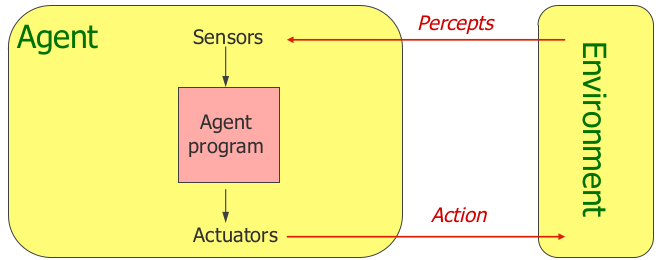
\includegraphics[width=6cm]{agent.png}
    \caption{Agent}
\end{figure}

\begin{description}

    \item[Agent]  :  Anything  that  can be  viewed  as  perceiving  its
    environment through sensor and acting through actuators.

    \item[Percept] : Refer to the agent's perceptual inputs at any given
        instant

    \item[Percept sequence] : Complet history of percept

\end{description}

\subsection{Concept of rationality}
\begin{description}

    \item[Rationality] : Is do the right think, but what is the
        right think for computer? Need \textit{Performance measure}

    \item[Rationnal  agent]  : For  each  possible  percept sequence,  a
    rational agent should select an  action that is expected to maximize
    its performance measure, given the  evidence provided by its percept
    sequence and whatever build-in knowledge the agent has.


   \item What is all the time rationnal :
        \begin{enumerate}
            \item Performance measure that define the criterion of success
            \item Knowledge of the environment by the agent
            \item Action that the agent can perform
            \item Percept sequence up to date
        \end{enumerate}

    \item The performance of an agent is measured by the sequence of action that it does. If the sequence is
    		desirable, then it performs well.
    \item Note : Rationnality $\neq$ omniscience, (expected performance $\neq$ actual performance)

    \item[Omniscience agent] : know the \textbf{real} result of its action.

    \item[Autonomy] :  An automous agent learn what it can do to compensate for partial or incorrect prior
    knowledge. (It shouldn't only rely on its prior knowledge)

\end{description}


\subsection{Nature of environments}
Task environnement (PEAS) is a specification to the \textbf{P}erformance,
\textbf{E}environment, \textbf{A}ctuators ans \textbf{S}ensors.

\begin{tabular}{|p{0.17\linewidth}||p{0.17\linewidth}|p{0.17\linewidth}|p{0.17\linewidth}|p{0.17\linewidth}|}
    \hline
    \textbf{Agent Type} & \textbf{Performance Measure} & \textbf{Environment} &
    \textbf{Actuators} & \textbf{Sensors} \\
    \hline
    \textbf{Medical diagnosis system} & Healthy patient, reduced costs &
    Patient, hospital, staff & Display of questions, tests, diagnoses,
    treatments, referrals & Keyboard entry of symptoms, findings, patient's
    answers \\
    \hline
    \textbf{Satellite image} & Correct image categorization & Downlink from
    orbiting satellite & Display of scene categorization & Color pixel arrays \\
    \hline
    \textbf{Part-picking robot} & Percentage of parts in correct bins & Conveyor
    belt with parts; bins & Jointed arm and hand & Camera, joint, angle
    sensors\\
    \hline
    \textbf{Refinery controller} & Purity, yield, safety & Refinery, operators &
    Valves, pumps, heaters, displays & Temperature, pressure, chemical sensors\\
    \hline
    \textbf{Interactive English tutor} & Student's score on test & Set of
    students, testing agency & Display of exercises, suggestions, corrections &
    Keyboard entry \\
    \hline
    \textbf{Taxi driver} & Safe, fast, legal, max profit & Roads, other traffic,
    customer, pedestrians &  Accelerator, display,  brake, signal  & Cameras,
    sonar, speedometer, FPS,\ldots \\
    \hline
\end{tabular}

The properties of the environment are the following:
\begin{description}
\item[Fully observable vs Partially observable :] All relevant information are accessible (chess vs poker)
\item[Single agent vs Multiagent:] Are there more than one agent, if yes
    then it can be a cooperation or a competition. (crossword puzzle vs chess)
\item[Deterministic vs Stochastic:] (chess vs poker)
    \begin{itemize}
        \item The next state of the environment depends entirely on the action of the
agent.
        \item Environment for the agent is less deterministic because
            he doesn't have all informations on the environment. (Cannot precisely
            determine the next state because of chance)
    \end{itemize}
\item[Episodic vs Sequential:] Experience of the agent is divided into atomic episode that are independent
from each other.
\item[Static vs Dynamic:] The environment can change while the agent is thinking. If the performance of the
agent change over the course of time, then its \textbf{Semidynamic}.(crossword vs chess with clock)
\item[Discrete vs Continuous:] The number of distinct states is finite and the sets of action and percepts are
discrete. (chess vs taxi driving)
\item[Known vs Unknown:]  The outcome for each action is given. Not the same as fully observable,for
example video games, know all the information via the screen but don't know what the button does.

\end{description}
\noindent
\begin{tabular}{|m{0.15\linewidth}|llllll|}
    \hline
    \textbf{Task Environment} & \textbf{Observable} & \textbf{Agents} & \textbf{Deterministic} & \textbf{Episodic} & \textbf{Static} & \textbf{Discrete} \\
    \hline
    \hline
    Crossword puzzle & Fully & Single & Deterministic & Sequential & Static & Discrete \\
    Chess with a clock & Fully & Multi & Deterministic & Sequential & Semi & Discrete \\
    \hline
    Poker & Partially & Multi & Stochastic & Sequential & Static & Discrete \\
    Backgammon & Fully & Multi & Stochastic & Sequential & Static & Discrete \\
    \hline
    Taxi driving & Partially & Multi & Stochastic & Sequential & Dynamic & Continuous \\
    Medical diagnosis & Partially & Single & Stochastic & Sequential & Dynamic & Continuous \\
    \hline
    Image analysis & Fully & Single & Deterministic & Episodic & Semi & Continuous \\
    Part-picking robot & Partially & Single & Stochastic & Episodic & Dynamic & Continuous \\
    \hline
    Refinery controller & Partially & Single & Stochastic & Sequential & Dynamic & Continuous \\
    Interactive English tutor & Partially & Multi & Stochastic & Sequential & Dynamic & Discrete \\
    \hline
\end{tabular}

\subsection{Structure of Agent}
An agent is composed of two parts:
\begin{itemize}
\item The \textbf{architecture} which is the computer device on which the agent is running.
\item The \textbf{program} which is a function that map the percepts to the action.
\end{itemize}
In general, the architecture makes the percepts from the \textbf{sensors} available to the program, runs the
program, and feeds the action choices of the program to the actuators as they are generated.

There exists different kind of agent:
\begin{description}
\item[Table-driven] a table of percepts and a function that maps each action
    to a percept.
\item[Simple reflex] agent that act depending on the current percept. Based on a condition-action
rule.
\item[Model-based reflex agent] keeps an internal representation of the
    environment.
\item[Goal-based] same as model-based except that the agent keeps a set of
    goal states.
\item[Utility-based] uses a utility function to choose between states.
\item[Learning] update its behaviour by experience. It should be able to know how it performs.
\end{description}
\section{Chapter 3 : Solving Problems by Searching}

\subsection{Key principles}

\begin{description}
    \item[Search] process of looking for a (or the best) sequence of actions, that leads to a goal (specific state of the environment), starting from an initial state
    \item[States] distinguishable stages during the problem solving process (representation of physical configuration)
    \item[State space] is a graph representation of the successor function with the cost.
    \item[Initial state] The state that the agent starts in.
    \item[Action] an action transports the agent from one state to another one by applying an \textit{operator}
    to a state
    \item[Transition model] A function that returns the state that results
        from doing action $a$ in state $s$
    \item[Successor] Any state reachable from a given state
    \item[Path] Sequence of state connected by a sequence of action.
    \item[Operators] possible ways to modify states in a given problem.
    \item[Goal test] A test that specify if a given state is a final result.
    \item[Step cost] numeric cost of taking action $a$ in state $s$ to get
        to $s'$.
    \item[Path cost] A function that assigned a numeric cost to each path.
    \item[Solution] a solution is a sequence of actions leading from the initial state to a goal state.
    \item[Optimal solution] an optimal solution has the lowest path cost among all solutions
    \item[Node] data structure constituting part of a search tree/graph and representing a state.
    \item[Frontier] set of generated nodes, which ancestors have been goal-tested (visited)
\end{description}

\subsection{Problem solving agents}

\textit{An  agent with  several immediate  options of  unknown value  can
decide what to do by first  examining future actions that eventually lead
to states of known value}

\paragraph{Assumption} : Environment is  static, deterministic, fully
observable and discrete.

\subsubsection{Problem definition}
A problem can be defined :
\begin{enumerate}
    \item States and \textbf{initial state}
    \item A description of the  \textbf{possible actions} available to the
    agent.
    \item A description of what each action does, called \textbf{transition
        model}.
    \item A \textbf{Goal test}
    \item A \textbf{Path cost} that use a step cost.
\end{enumerate}

\subsubsection{Solution}
A  \textbf{solution}  is a  sequence  of actions  leading
from  the  initial state  to  a  goal state. An  \textcolor{red}{optimal}
\textbf{solution} has the lowest path cost amoung all solutions.

\subsubsection{State space}
Together, initial  state, actions and transition model define
\textbf{state space} of the  problem. (\textit{Graph representation of
the successor function with the cost})

\subsubsection{Abstraction}
Removing detail from a representation of the state or the action.

\subsection{Example}
For eight puzzles
\begin{itemize}
\item The state is the position of all the 8 tiles and the empty one.
\item The initial state is a random, any state can be the initial one.
\item The action are simply moving the blank space in four directions: up, down, left and right.
\item The transition model returns the effect of moving the blank space in
    one of the four directions.
\item The goal test is to check if the state is in the wanted configuration. (tiles in order)
\item The step cost is one, so the path cost is the number of step done in the path.
\end{itemize}

\subsection{Searching for Solutions}

\begin{description}

    \item[Searching] for solutions  is a traversal of  some search space
    from the \textit{initial  state} to the \textit{goal  state} using a
    legal sequence of actions (as defined by operators).

    \item[Expanding] : apply each legal action to current state (=
        generating states)

    \item[Frontier] : set of all leaf nodes available for expansion.
        (That corresponds of all leaf nodes which ancestors have visited)

    \item[Explored set] : set of all nodes previously visited.
\end{description}

\paragraph{Loopy path} A  complete search tree can be infinite if there
is  looping. But  we  don't consider  this one  because  path cost  are
additive and  step cost are  non-negative. (\textit{Loopy path  is never
better than same path without loop})

\subparagraph{ } To avoid redundant path, we use \textbf{graph search}
by using \textit{explored set}

\subsubsection{Tree and Graph Search}

There are two ways to perform the search\footnote{the slides specifies an
algorithm to search in a tree}.

\begin{itemize}
    \item \textbf{A graph representing the state space}: you represent
all the possible states as a graph, and you move between those states
    \item \textbf{A search tree}: you list all the possibilities from
the current states using the possible \textit{operators}
\end{itemize}

\subsubsection{States and Node}
\begin{itemize}
    \item A \textbf{state} is a representation of a physical
        configuration that represents a intermediate state.
    \item A \textbf{node} is a data structure constituting part
        of a search tree
\end{itemize}

So, there can be many nodes with same state!

\subsubsection{Repeated States}

Failure  to detect  repeated states  can turn  a solvable  problems into
unsolvable ones. We are going to  avoid visiting nodes that have already
been visited.

Use \textbf{graph search} is like tree  search but do not  expand nodes
with a state appearing in an already visited node.

\subsubsection{Algorithm description}
For the tree search
	\begin{enumerate}
	\item Initialize the frontier with the initial state
	\item Loop
		\begin{enumerate}
			\item If the frontier is empty then return failure
			\item Choose a state in the frontier
			\item Check if goal test (if yes return solution path), if not expand it and add resulting state in the
			frontier
		\end{enumerate}
\end{enumerate}
For the graph is the same except that it keeps an exploring set (contains
the nodes visited) and does not expand the node if it's already in the exploring set.
\subsubsection{Search strategies}

There is two types of search: \textbf{uninformed search} where the only
information known by the agent is \textit{Am I  on the goal?}  and the
\textbf{informed search} where agent has a background information about
the problem.

We can evaluate a search strategy with 4 criteria:
\begin{itemize}
    \item \textbf{Completeness}: it finds a solution if one exists
    \item \textbf{Time complexity}: usually in terms of the number of nodes generated/expanded
    \item \textbf{Space complexity}: maximum nodes in memory
    \item \textbf{Optimality}: it finds a least cost solution?
\end{itemize}
And you use 3 different variables:
\begin{itemize}
    \item $\textbf b$  maximum branching factor of the search tree (the maximum number of subnodes)
    \item $\textbf d$  depth (in the tree) of the least-cost solution
    \item $\textbf m$  maximum depth of the search tree (may be infinite)
\end{itemize}



\subsection{Uninformed search}
Here will be presented multiple algorithms to search in a tree.

\begin{figure}[!ht]
\centering
\begin{tabular}{|l|m{2cm}|m{2cm}|m{2cm}|m{2cm}|m{2cm}|m{2cm}|}
\hline
& \textbf{BFS} & \textbf{UCS} & \textbf{DFS} & \textbf{DLS} & \textbf{IDS} & \textbf {BDS}\\
\hline
& level by level & cheap path & last depth & limited depth & iterative depth & bi direct  \\

\hline
\hline
\textbf{Complete} & \textcolor{red}{if} \textbf{b} finite & \textcolor{red}{if} \textbf{sp} > 0  & NO  & \textcolor{red}{if} $l\geq d$ & YES & YES\\
\hline
\textbf{Optimal} & \textcolor{red}{if} \textbf{sc} = 1 & YES & NO & \textcolor{red}{if} l==d & \textcolor{red}{if} += 1 & \textcolor{red}{if} \textbf{sc} = 1 \\
\hline
\textbf{Time} & $b^{d+1}$    & $b^{1 + C/\epsilon}$ & $b^m$ & $b^l$ & $b^d$ & $b^{d/2}$\\
\hline
\textbf{Space} & $b^{d+1}$ & $b^{1 + C/\epsilon}$ & $bm$ & $bl$ & $bd$ & $b^{d/2}$ \\
\hline
\textbf{Frontier} & FIFO & Priority & LIFO & LIFO & LIFO & FIFO \\
\hline

\end{tabular}
\caption{Uninformed Search Algorithm}
\end{figure}


\subsubsection{Algorithm: Breadth-First Search}
The goal is to search in a tree level by level from \enquote{left} to
\enquote{right}.

The memory use grows really fast!

You start from the root node and adds the subnodes at the end of a
\textcolor{red}{FIFO queue} (the queue being the \textit{frontier}).

\paragraph{Criteria} \textit{Complete} if b is finite and \textit{optimal} if the cost per
step is 1 (but in general use it ain't \textit{optimal}).

\paragraph{Complexity} \textit{Time complexity} of $O(b^d)$\footnote{Time complexity: $1+b+b^2+...+b^d+b(b^d-1) = O(b^{d+2}) = O(b^d)$} and a \textit{space complexity} of $O(b^d)$.

\begin{figure}[!ht]
    \centering
    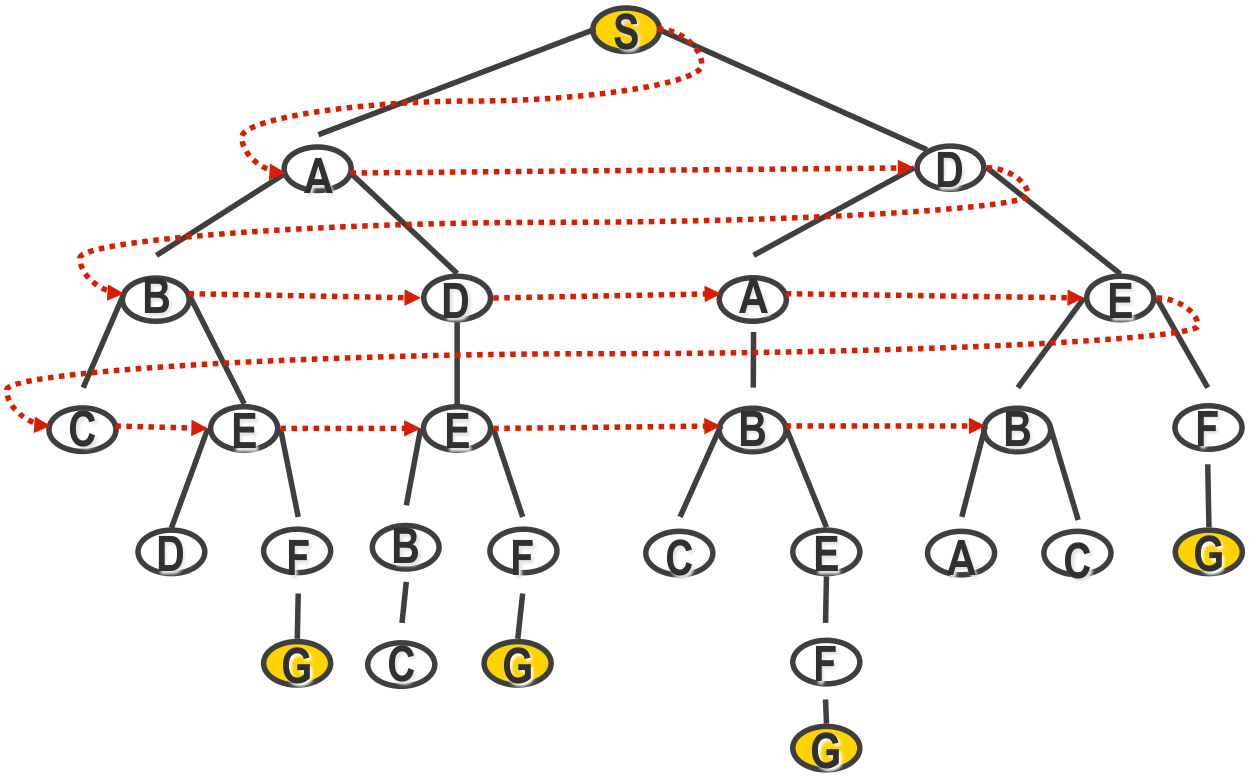
\includegraphics[width=0.4\linewidth]{breadth_first_search.png}
    \caption{Representation of a BFS in a tree}
\end{figure}

\subsubsection{Algorithm: Uniform-Cost search}

Like a BFS but this is not the shortest path but the \textbf{cheapest} path.

This is similar to Breadth-First but with a cost added to the reachable
nodes. The frontier is handled as a priority queue where the node with the minimum step cost is expanded first.

The \textit{path cost} is simply the sum of the individual edge
costs  to reach the current node. \textit{Frontier} is now a queue
ordered by the path cost.

\paragraph{Criteria}
This algorithm is \textit{optimal} compare to Breadth-First, it is
\textit{complete} if step cost is strictly positive to avoid the infinite path with zero-cost action.

\paragraph{Complexity}

\textit{time and  space complexity}  are difficult to establish because
\textit{uniform cost search} are guided by path costs rather than depth.
(So it explores large trees of small steps before
exploring paths involving large and perhaps useful step.)

We evaluate it with $O(b^{C/\epsilon}$.\footnote{$C$ is the cost of the optimal solution and $\epsilon$ the step cost strictly positive}

\subsubsection{Algorithm: Depth-first Search}

The \textit{frontier}  is implemented as a  \textcolor{red}{LIFO queue}.
Concretely, we visit a branch of the tree until we reach the leaf, then we
start back for another branch.

\paragraph{Criteria}
This algorithm isn't \textit{complete}, as you can fall in infinite depth
spaces. The \textit{time complexity} is $O(b^m)$

\paragraph{Complexity}
The \textit{space complexity} is $O(mb)$. \textbf{It is not an \textit{optimal} algorithm}.

\subsubsection{Algorithm: Depth-Limited Search}

It is the same as a \textit{Depth-first} but with a depth-limit $l$ and
then replace $m$ by $l$.

Cannot find a solution if $l < d$ !

\subsubsection{Algorithm: Iterative Deepening}

Let $l$ be  a limit. This algorithm is a Depth-Limited, but we increase
the depth limit as we search. It combines advantage of Breadth-First and
Depth-First methods. With this technique,  many nodes are visited multiple
times but it doesn't really matter because the number of those nodes is
\enquote{small}.

\paragraph{Criteria} This algorithm is \textit{complete} and this is an
\textit{optimal} algorithm if we increase one by one.

\paragraph{Complexity} It has a \textit{time complexity} of $O(b^d)$ and
a \textit{space complexity} of $O(bd)$.


\subsubsection{Algorithm: Bidirectional Search}

We use two Breadth-First search (start to goal and goal to start) and we stop when two search trees
intersects. There is a few difficulties with this type of search:

\begin{itemize}
    \item Predecessors of a (goal) state must be generated. (Not always possible)
    \item Search must be coordinated between the two search processes
    \item What if multiple goal states?
    \item One search must keep all nodes in memory
\end{itemize}

\paragraph{Criteria} This algorithm is \textit{complete}  and it's an
optimal algorithm is step cost is 1 (like in Breadth-First).

\paragraph{Complexity} It has a \textit{time complexity} of $O(b^{d/2})$
and a \textit{space complexity} of $O(b^{d/2})$.

%\begin{tabular}{|l|p{0.12\linewidth}p{0.12\linewidth}p{0.12\linewidth}p{0.12\linewidth}p{0.12\linewidth}p{0.12\linewidth}|}
%    \hline
%    Criterion & Breadth-First & Uniform-cost & Depth-first & Depth-limited & Iterative deepening & Bidirectional search \\
%    \hline
%    Completeness & Yes* & Yes* & No & \textcolor{red}{if $l \ge d$} YES & YES & YES* \\
%    Time & $b^{d+1}$ & $b^{C*/e}$ & $b^{m}$ & $b^{l}$ & $b^{d}$ & $b^{d/2}$ \\
%    Space & $b^{d+1}$ & $b^{C*/e}$ & $bm$ & $bl$ & $bd$ & $b^{d/2}$ \\
%    Optimality & YES* & YES* & NO & NO & YES & YES \\
%    \hline
%\end{tabular}

\subsection{Informed search}

\begin{description}
    \item[Informed search] we search using problem specific knowledge and find and/or deduce information about future states and future paths. (\textit{exploit informations on the node
        to make better decision})
\end{description}


\begin{figure}[!ht]
    \centering
    \begin{tabular}{|l|m{2.5cm}|m{2.5cm}|m{2.5cm}|m{2.5cm}|m{2.5cm}|}
        \hline
        & \textbf{GBFS} & \textbf{A*} & \textbf{IDA*} & \textbf{RBFS} & \textbf{SMA*} \\
        \hline
        & best solution & total estimated & A* with iterative deepening & \\

        \hline
        \hline
        \textbf{Complete} & No (loop) & \textcolor{red}{if} $\epsilon$ > 0 & Yes  \\
        \hline
        \textbf{Optimale} & NO & \textcolor{red}{if} admissible, consistante & \textcolor{red}{if} admissible, consistante\\
        \hline
        \textbf{Time} & $b^m$ & $b^m$ & Exponential\\
        \hline
        \textbf{Space} &$b^m$ & $b^m$ & Linear\\
        \hline
        Frontier & Priority & Priority &Priority &\\
        \hline
    \end{tabular}
    \caption{Informed Search Algorithm}
\end{figure}


\paragraph{Best-first search}

is a general search algorithm (Tree or graph) in which a node is selected
for expansion based  on  an \textbf{evaluation function} ($f(n)$).  This
function is  construed as an  \textit{estimated cost}\ldots so  the lowest
evaluation is expanded first. So we use \textcolor{red}{priority queue}.

Take care that  this is an \textbf{evaluation}  function \textbf{not the
exact} distance.\footnote{If it was the exact distance, we would already
know if we are (or not) on the solution path, and we would never have to
change direction at any point during the search.}

\subsubsection{Heuristics functions}

A \textbf{heuristic function}, denoted $h(n)$, is the estimated cost of the node to the goal.\footnote{$f(n)=g(n)$} Obviously we don't know this cost, so we'll have to approximate it. You have to define the heuristic function for each problem you'll have to solve.(They're problem specific)

\begin{description}
    \item[Contour] a contour is a set of nodes with $f(n) \leq$ some fixed value

    \item[Optimistic heuristic] an admissible heuristic because they think the cost of solving the problem is less than it actually is

    \item[Admissible heuristic] it never overestimates the cost of reaching
        the goal, i.e. the cost it estimates to reach the goal is not
        higher than the lowest possible cost from the current point in the
        path.\cite{wikiadmheur} $h(n)$ = 0 if is a goal state. (ex:Manhattan distance in a maze)

    \item[Consistent heuristic] The estimation from a node $n$ to the goal, is lesser than the cost\footnote{Not an estimation, the exact cost} from $n$ to a new node $n'$ with the estimation from the node $n'$ to the goal $$h(n) \leq c(n,a,n')+h(n')$$
        Consistent heuristic is admissible.

    \item[Triangle inequality] : Each side of a triangle cannot be longer than the sum of
        the other two sides. \\
        \begin{tabular}{m{8cm}m{7cm}}
            \begin{itemize}
                \item h(n) : estimated cost between n and G
                \item C(n, a n') : cost to go in n' from n with action a
                \item h(n') : estimated cost between n' and G
            \end{itemize}

                    &
        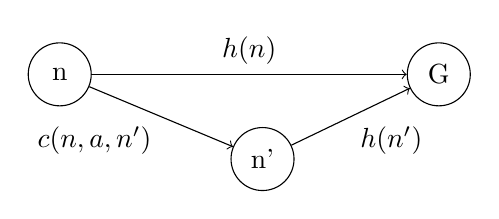
\begin{tikzpicture}
            \node[circle, draw, minimum size=0.8cm,] (N) {n};
            \node[circle, draw, minimum size=0.8cm, below right = 0.5cm and 2cm of N] (NN) {n'};
            \node[circle, draw, minimum size=0.8cm, right = 4cm of N] (G) {G};

            \path (N) edge[->] node[below left] {$c(n, a, n')$} (NN) ;
            \path (NN) edge[->] node[below right] {$h(n')$} (G) ;

            \path (N) edge[->] node[above] {$h(n)$} (G) ;

        \end{tikzpicture}
    \end{tabular}


    \item[Monotonicity] If $h(n)$ is consistent (Let a be an action and n,n'
    two nodes we  have $h(n) \leq c(n,a,n') + h(n')$)  then $f(n)$ along any
    path is non decreasing.

        Suppose that $n'$ is successor of $n$. We have
        \begin{eqnarray*}
            g(n') &=& g(n) + c(n,a,n')\\
            f(n') &=& g(n') + h(n')\\
            &=& g(n) + c(n,a,n') + h(n')\\
            c(n,a,n') +h(n') &\geq& h(n)\\
            g(n) + c(n,a,n') + h(n') &\geq& g(n) + h(n)\\
            &\geq& f(n) \\
            f(n') &\geq& f(n)
        \end{eqnarray*}
\end{description}

\paragraph{Note:}
	\begin{itemize}
		\item if $h(n)$ is consistent then $f(n)$ is non-decreasing.
		\item if $h(n)$ is consistent then $h(n)$ is admissible and A* is optimal
	\end{itemize}
\subsubsection{Algorithm: Greedy Best-first search}
GBFS tries to expand the node that is \textbf{closest} to the goal.
(\textit{For path finding, the straight-line distance})

\paragraph{Criteria} It's not a optimal solution and it's no complete
because you can loop.

\paragraph{Complexity} The \textit{space} and \textit{time} complexity
is $O(b^m)$ but with a good heuristic the complexity can be reduced
substantially.


\subsubsection{Algorithm: A* search}
Minimizing the total estimated solution cost (fusion Greedy and uniform-cost).

A* uses the distance and adds the current solution path cost. Let $g(n)$
be the cost of the solution going to the node $n$ and $h(n)$ a heuristic
function. $$f(n)  = g(n)  + h(n)$$ $h(n)$  must never  overestimates the
cost to reach a goal (and  so $f(n)$ also never overestimates the cost).
If $n$ is the goal node, then $h(n) = 0$.

\paragraph{Complexity}

\textit{space} and \textit{time} are $O(b^d)$  This is a nice algorithm,
but we have  a \textcolor{red}{space complexity issue}, it takes a lot of
memory!

\paragraph{Criteria} It's \textit{complete} if the cost cannot be negative
to avoid infinite zero-cost action.
It's optimal if heuristic is admissible (\textit{in tree search}) or
consistent (\textit{in graph search}).

\paragraph{Properties of A*}

Here are the properties of A*:
\begin{itemize}
    \item With $h(n)$ consistent, the sequence of nodes expanded by A* using \textbf{Graph-Search} is in non decreasing order of $f(n)$
    \item A* (using \textbf{Graph-Search}) is optimal if $h(n)$ is consistent
    \item A* expands all nodes with $f(n) \leq C^*$ ($C^*$ being the optimal cost)
    \item A* expands some (at least one) of the nodes on the $C^*$ contour before finding the goal
    \item A* expands no nodes with $f(n) > C^*$
\end{itemize}

A* is \textbf{optimally efficient} because he doesn't expand node with
$f(n) > C*$. We  can't be more efficient because if we don't expand all
nodes with $f(n) < C*$ we take the risk of missing the optimal solution!


\paragraph{To proof of A* optimality}


we just prove that A* expands no nodes with $f(n) > C^*$ .
\begin{enumerate}

    \item Let  $G$ be  a goal node  in the fringe,  but in  a suboptimal
    path. Its path cost $g(G)=C$ is not the lowest one\footnote{$\exists
    C^* : C  > C^*$}.

    We use the  formula at line (1), then as  $G$ is a
    goal node and $h$ is admissible we have line (2).

        \begin{eqnarray}
            f(G) &=& g(G) + h(G)\\
            \footnotemark\quad h(G) &=& 0 \\
            f(G) &=& g(G) = C > C^*\\
            \color{red}f(G) &\color{red}>&\color{red} C^*
        \end{eqnarray}
        \footnotetext{Because G is a goal state}

    \item Let $n$ be a node in the fringe, with $n$ in the path to the optimal soluation (cost $C^*$). As $h$ is admissible, we have $f(n) = g(n) + h(n) \leq C^*$. Then we have
    $$f(n) \leq C^* < f(G)$$
    In this scenario, $G$ will never be selected, so the hypothesis is absurd.
\end{enumerate}

In conclusion \textbf{A* expands no nodes with} $f(n) > C*$.

\subsubsection{Memory-bounded heuristic search}

Complete and optimal with an exponential complexity for \textit{time} and
linear complexity for \textit{space}

\paragraph{Algorithm: Iterative Deepening A* (IDA*)}

We combine the algorithm A* with the Iterative deepening. Let $l$ be a limit.

IDA* use f-cost(g+h) as a cutoff rather than the depth. At each iteration,
the cutoff-value is the smallest f-cost of any node the exceeded the cutoff on
the previous iteration.

\subparagraph{Complexity} Complete and optimal with complexity exponential for \textit{time}
and linear for \textit{space}

It's a nice algorithm, but we can still improve the algorithm. With an
infinite amount of memory, A* would be the best algorithm. If I agree to
re-do some operations IDA* is the best.

So we use A* and when we
are  short of  memory we switch to IDA*.\footnote{We called this one
\textit{Simple memory-bounded A*}}


\paragraph{Algorithm: Recursive best-first search}
It's a simple recursive algorithm trying to run in a linear space. The structure is
the same than the DFS except it does not keep going down indefinitely.\\
It uses a $f_{limit}$ value variable to keep track of the f-value of the best alternative path
from the ancestor of the current node.


\paragraph{Algorithm: Memory-bounded A* and simplified MA*}
SMA* does run as A* until the memory is full. When the memory is full, it
needs to discard a node if it wants to add a new one. It will discard the
worst one (one with highest f-value).\\
SMA* backups the value of the its parent so that the ancestor knows the quality of the best
path in that subtree.


\subsubsection{Learning to search better}
\begin{description}
\item [metalevel state space:] Each state captures the internal state of a program that is searching in
a object-level-space. For example in A*, the internal state is the current search tree.
\end{description}
By keeping the internal state, metalevel learning algorithm know from experience the unpromising
subtrees.

\subsection{Heuristic in practice}

\subsubsection{Comparing two heuristics}

To compare two heuristics you may use:
\begin{itemize}
\item The number of generated nodes $N$
\item The effective branching factor $b^*$, with $N+1 = 1 + b^* + (b^*)^2 + ... + (b^*)^d$ (an ideal $b^*$ is close to one)
\end{itemize}

\subsubsection{Designing heuristics}

You must choose an \textit{admissible} and \textit{consistent} heuristic. You must choose the most dominant heuristics\footnote{The most dominant is the one with the most informations}.


\section{Chapter 4.1 : Local Search}

A search  is the operation of  looking for a solution  where solution is
a path from start to goal.  We've  seen  two  kinds  of  search,  an
\textit{uninformed search} in which no prediction is available about the
cost of the path and \textit{informed search}, where we can estimate
the cost of the solution.

\paragraph{ }
\textbf{Local search} will not keep track of paths because it just want
to have a goal, it only keeps the current path :
\begin{itemize}
    \item Use a small amount of memory,
    \item They can find solution in infinite search,
    \item They find a reasonable (\textit{not optimal}) solution.
\end{itemize}

\subsection{How does it work?}

You always \textbf{improve the current solution} (\textit{Store one solution at each iteration})
The next solution is found in the \textbf{neighborhood} of the current solution.

Typically modify the value of a variable at each step.

\subsection{Optimization Problem}

We have an \textbf{objective function} that you can \textit{minimize} or
\textit{maximize}.  You want  to find the  global maximum/minimum.  Ex:
\textit{distance to position}, \textit{number  of queens attacking in the
8 queens problem},\ldots

The only  problem of this algorithm are \textbf{local optimal}, so you
may be stuck at some point in the search.

\begin{figure}[!ht]
    \centering
    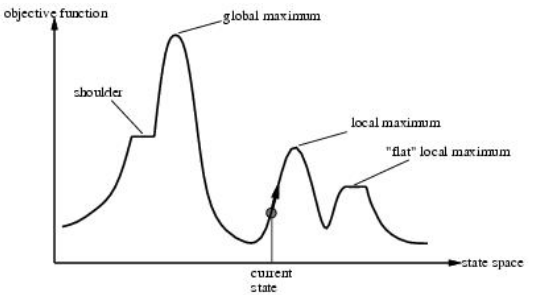
\includegraphics[width=7cm]{local.png}
    \caption{Objective function on the state space}
\end{figure}

\subsubsection{Neighbourhood}

\paragraph{Size}
If we choose  to take larger neighbourhood we  will have \textit{shorter
path}  to the  solution, but  we will  also need  \textit{more time}  to
explore all possibilities. It's a \textbf{key design decision} (\textit{choice
between length of path and exploration})

\paragraph{Connectivity}

From each solution there is a path to an optimal solution. It has two
advantages:
\begin{itemize}
    \item Required for convergence property
    \item No need of restarting strategy (you will never be block)
\end{itemize}

\paragraph{Constraint}

Two approaches are possible to combine faisability with optimality requirements :
\begin{itemize}
\item
	\begin{enumerate}
	\item Maintain feasibility at all times
	\item Explore only feasible solutions
	\end{enumerate}
\item
	\begin{enumerate}
	\item Do not maintain feasibility at all time; relax a subset of the constraints
	\item Explore a larger search space
	\item Drive the search to high quality and feasible solutions
	\end{enumerate}
\end{itemize}

\subsection{Heuristics and metaheuristics}

\begin{description}

    \item[Heuristics] focus on  choosing the next solution and drive the
    search towards \textit{local  optimum} based  on local information
    (\textit{current solution and its  neighborhood}). It's a memoryless
    solution.

        \begin{itemize}
            \item Hill-climbing
            \end{itemize}

    \item[Metaheuristics] Try to escape from  local and drive the search
    towards  \textit{global optimality}  based on  collected information
    on  the   execution  sequences.  It  includes   memory  or  learning

        \begin{itemize}
            \item Iterated local search
            \item Simulated annealing
            \item Guided local search
            \item \ldots
            \end{itemize}

    \item[Systematic heuristics]  Exploration (possibly partial)  of the
neighborhood to determine the next solution

\end{description}

\subsection{Algorithm: Hill climbing}

Move on the direction of increasing value and stop the iteration when
it's impossible to go further.

This algorithm go quickly to a best solution but he have multiple issues :
\begin{itemize}
    \item Local maximum
    \item Plateau : \textit{a maximum flat area} can stop the algorithm (solution:
        make a number limit where iteration have same value)
    \item Ridges : sequence of local maxima where Hill climbing are very difficult to navigate
\end{itemize}


Hill climbing depend  very  much on  the  shape  of  the state-space  landscape!  Hill
climbing has a  big Achilles hell, the local maxima. You cannot escape
local maxima,  considering that  hill climbing \textbf{will never makes
downhill moves}.

\subsubsection{Variants}

There is multiple variants of the hill climbing algorithm:
\begin{description}
    \item[Stochastic hill climbing] randomly choose in the list of uphill moves
    \item[First-choice hill climbing] pick the first good successor you find
        (\textit{useful when there is a large amount of possibilities})
    \item[Random restart] You start from multiple random points
\end{description}


\subsection{Random walks}

You can consider another kind of heuristic, in which you select randomly
an  element of  the  neighborhood and  decide whether  to  accept it  as
the  next solution.  There  is two  possibles approaches:  \textit{random
improvement}  and  \textit{metropolis heuristic}.

\subsection{Simulated annealing}

Algorithm that combine Hill Climbing, a scheduler and a metropolis step.
\begin{itemize}
    \item Scheduler : Is used to link a explicative variable with a probability to accept a
        downhill value
    \item Metropolis step : is the step where we select a downhill value with a probability
\end{itemize}

The algorithm starts by randomize hard and then gradually reduces the intensity of randomized
and take more the best solution in neighborhood.

(\textit{Annealing is the process of heating metal and letting it cool slowly to lock in the stable locations of the molecules} )

So here is the principle of this technique:
\begin{enumerate}
	\item Always move uphill if possible (hill climbing)
	\item Sometimes go downhill (like in metallurgy when temperature is high).
	\item Optimality is guaranteed with slow annealing schedule.
\end{enumerate}


\subsection{Local beam search}

Hill climbing and simulated annealing techniques keep one state in memory.
In this technique you keep $k$ states in memory and at each step all states
generate successors and we take the $k$ best one.

(\textit{Information between states can be shared, like
\enquote{Come over here, the grass is greener}}).
In practice, local beam search suffer from a lack of diversity because
state quickly become concentrated in a small region.


\paragraph{ } A stochastic beam search (like stochastic hill climbing)
help to alleviate this problem


\subsection{Genetic algorithms}

Based on theory  of evolution, start with  k initial  state(s).
(\textit{population})  and the  next  generation are produced by merging
between individuals from current population.

An individual is represented by a fixed-length string and its \textit{fitness}
(score for each state, greater is better) is evaluated.

\paragraph{Cross over} A cross over point is choose at each reproduction. (it's the position where
the pair will be merged)
The goal is to can produce s state that is long way from either parent state.
( ex: with cross over at point 3, AAACCCC and DDDEEEE $\to$ AAAEEEE and DDDCCC)


\paragraph{Random mutation } can also perform for explore new parts of
search space, but does this with a low probability to not break a good solution!


\paragraph{ }
Good compromise between go to the better, random exploration and shared information
between many state.
The only issues with this algorithm is that crossover is not applicable to all problems.

\subsection{Tabu search Metaheursitics}
You select  the best  neighbor that  has \textbf{not yet}  been visited  and only
maintain a suffix of the sequence visited node, not all of them.

An abstraction is used to represent the suffix (to reduce the memory). We change the suffix
if the move improve the best solution so far.

\subsection{Intensification vs Diversification}
\begin{tabular}{m{8cm}|m{8cm}}
Intensification & Diversification \\
\hline

	\begin{description}
		\item[Goal] increase search around promising areas
		\item[Risk] premature convergence
		\item[Mean] favor good solutions
	\end{description}
&
	\begin{description}
		\item[Goal] explore new ares
		\item[Risk] convergence to optimality may be too long
		\item[Mean] probabilistic choice of solutions
	\end{description}
\end{tabular}

\subsection{Other local search Approaches}

There is a bunch of other local search:
\begin{description}
    \item[Variable Neighborhood Search] sequence of neighborhood
    \item[Guided local search] use a sequence of objective functions to drive away from local optima
    \item[Adaptive local Search] The heuristics/metaheuristics are dynamically adapted during the search
    \item[Ant colony optimization] the selection function is updated
    \item[Statistic Local Search] another name for Local search, stressing the stochastic aspect of the search
\end{description}



\section{Chapter 5 : Adversarial Search}

\subsection{Game}

\textbf{Game theory} view any multiagent environment as a game, provided that
the impact of each agent on the other is \textit{significant}.

In AI, the most common games are deterministic (\textit{fully observable with utility value at
the end of the game are always equal or opposite}), turn-taking, two-player, zero-sum game of
perfect information (if someone wins, the other loose).

There is also game with imperfect information and not deterministic value because of chance.


\textbf{A game} :
\begin{description}
    \item[Initial state] ($s_0$) and who is playing first.
    \item[Player (s)] : which player moved
    \item[Actions (s)] : set of legal moves
    \item[Result (s, a)] : \textit{transition model} which define result of a move
    \item[Terminal set (s)]
    \item[Utility (s,p)] : \textit{utility function} define the final
        numeric value for a game that ends in terminal state $s$ for a
        player $p$.
        \textit{zero-sum game} defined as one where the total payoff to all players is the same for every instance of the game.
\end{description}

\textbf{Game tree} : tree where nodes are game state and edges are move.

\begin{figure}[!ht]
\centering
\begin{tabular}{|l|m{3cm}|m{3cm}|m{3cm}|m{3cm}|}
\hline
& \textbf{MinMax} & \textbf{Prunning} & \textbf{H-MinMax} & \textbf{ExpectMin} \\
\hline
& All tree & with alpha-beta & Limited depth & Stochastic \\

\hline
\hline
\textbf{Complete} & \textcolor{red}{if} \textbf{tree} finite & \textcolor{red}{if} \textbf{tree} finite  & YES  & YES \\
\hline
\textbf{Optimal} & YES & YES & NO & NO \\
\hline
\textbf{Time} & $b^{m}$    & $b^{d/2}\textrm{ or }b^{3d/4}$ & $b^l$ & $b^m n^m$\\
\hline
\textbf{Space} & $bm$ & $bd/2\textrm{ or }3bd/4$ & $bl$ & $b^m$ \\
\hline

\end{tabular}
\caption{Adversarial Search Algorithm}
\end{figure}



\subsection{Optimal decision}
Given game tree, optimal strategy be determined from the minimax value of each
node \textit{assuming that both players play optimally}.

Minimax is perfect play for deterministic game and if the opponent doesn't play
optimally, he is better.

\begin{figure}[!ht]
    \centering
    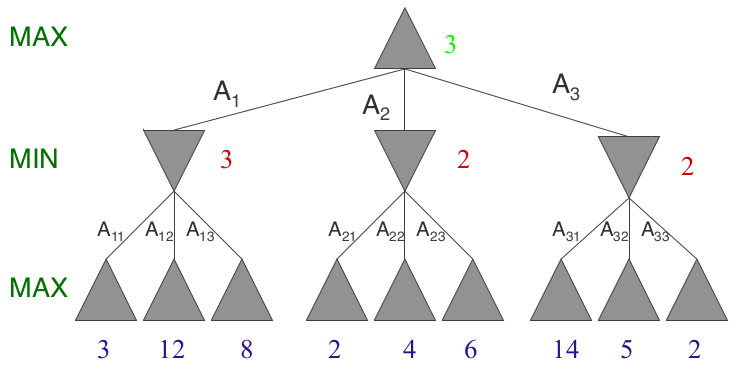
\includegraphics[width=10cm]{minmax.png}
    \caption{Minimax}
\end{figure}

\subsubsection{Algorithm: minimax}
Generate game tree to the terminal states and apply the utility function on these state.
After apply minimax to go on the top and value determine move.

Minimax is complete if tree is finite.

\paragraph{Complexity}
Such as minimax performs a \textcolor{red}{DFS} on the game tree, the
\textit{space} complexity is $O(bm)$
or $O(m)$ if action are generated one at a time.

\textit{Time} complexity is $O(b^m)$.

\subsubsection{Optimal decisions in multiplayer games}
When there are more than 2 players, we keep vectors at each node , where element of the vector are the
utility of each player. Each player will choose the move that maximize its utility function.

\subsection{Alpha-beta pruning}
\begin{figure}[!ht]
\begin{tabular}{m{10cm}m{6cm}}
    \centering
    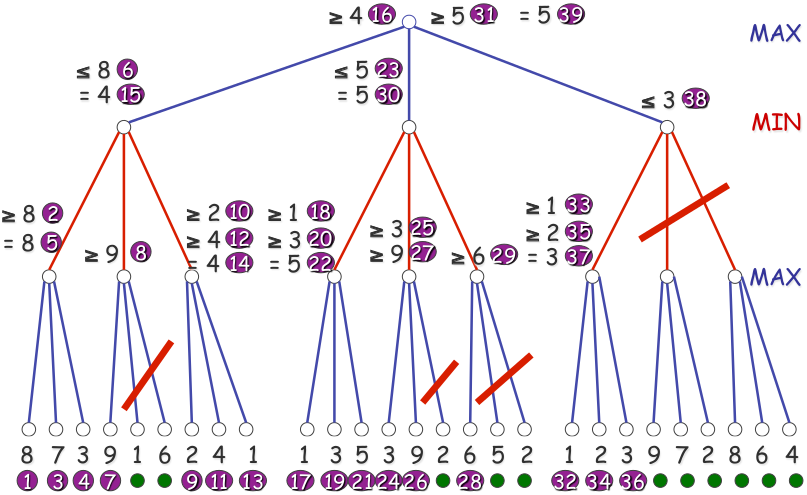
\includegraphics[width=10cm]{minmax_ex.png}
&

\begin{description}
    \item $\mathbf{\alpha}$ : value of the best (\textit{higher}) choice found
        so far at any choice point along the path for \textbf{MAX}
    \item $\mathbf{\beta}$ : value of the best (\textit{lowest}) choice found
    so far at any choice point along the path for \textbf{MIN}
\end{description}
\end{tabular}
\end{figure}

Pruning does not affect final result.

\paragraph{Complexity} if successors are ideally visited, \textit{time} complexity
is O($b^{(d/2)}$) and if visited randomly O($b^{3d/4}$)


\subsubsection{Move ordering}

Alpha beta pruning is highly dependent on the order in which the states are
examined.

\paragraph{Dynamic move ordering :} We can try the moves that were the best in the past and find the \textbf{Killer move}.

\paragraph{Game graph} There are repeated states in many games because of \textbf{transpositions}.
To be efficient, we can store the evaluation of state in hash table called \textbf{transposition
table}.

This table can doubling the reachable search depth in chess, but with a million node per second,
it's not possible to keep all nodes in table\ldots To solve this, various
strategies choose which nodes to keep and which nodes to discard.

\subsection{Imperfect real-time decisions}
In practice, make complete game tree is usually not practical.
So, program should cut off the search earlier and apply a heuristic \textbf{evaluation
function} on states in search to estimate the expected utility.

Change minimax :
\begin{enumerate}
    \item Utility function by heuristic evaluation function (\textsc{eval})
    \item Replace terminal set by a cutoff test that decide when apply \textsc{eval}
\end{enumerate}

\subsubsection{Evaluation function}
\begin{itemize}
    \item Must be consistent with the utility function.
    \item Trade-off between accuracy and time cost.
    \item Reflect the actual chances of winning.
    \item Weighted \textbf{linear function} are frequently used with a combination of features.
\end{itemize}

We used weighted linear function only if the feature are independent (For
example some pieces in the chess are more powerful at the end of the game
because there is more space). So some programs use non linear combinations
of features.


\subsubsection{Cutting off search}
The most straightforward approach is to set a fixed depth limit.
But there is an issue if the state is favorable to fast change in the next
state\ldots

\paragraph{Quiescent}  To solve this problem, the evaluation function
should be applied only to position that are \textbf{quiescent},  i.e.
stable state. (\textit{unlikely  to exhibit wild swings in  value in the
near future})

\paragraph{Horizon effect} We can delay disasters, but we don't prevent them. It could happen because of cut-off as the horizon is not deep enough.

If an agent is facing a move that cause serious damages and is unavoidable at the end, it will try to avoid it as long as possible. At the end this will end up losing as much or even more.

\subsubsection{Forward pruning}
Some moves at a given node are pruned immediately without further consideration.
It cuts off moves that you recognized as bad.

\paragraph{ } One approach is \textbf{beam search} : consider only at
\enquote{beam} of the $n$ best moves rather than all possible moves.


\subsubsection{Search vs Lookup}

For many games, table lookup are used for the  opening and end of the
game. Because at first (at  the end)  the situation are  very similar.
After  some moves,  the actual  search must  be done  because situation
differs.


\subsection{Stochastic games}
Stochastic games are games with a degree of unpredictability through random elements.

$\rightarrow$ Requires chance nodes in addition to the max/min nodes

\subsubsection{Expectminimax} Algorithm that adds chance nodes in addition
to the max/min nodes.

\paragraph{Complexity} \textit{time} complexity is $O(b^m n^m)$ where $n$
is the number of distinct chance events and \textit{space} complexity is $O(b^m)$

\begin{figure}[!ht]
    \centering
    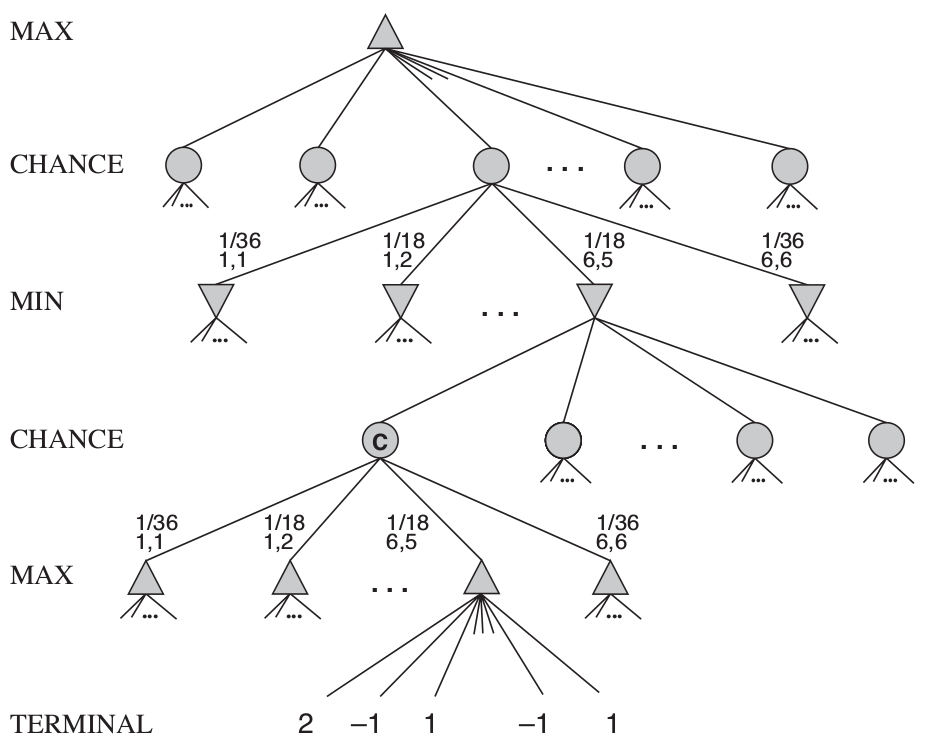
\includegraphics[width=0.5\linewidth]{stochastic.png}
    \caption{Game with dice node}
\end{figure}


\subsubsection{Evaluation  function for  game  of  chance}

The  evaluation function can be totally different if we change  the
random event.  So, the \textbf{evaluation  function} must be  a positive
linear transformation  of the  probability of  winning from  a position.
(\textit{more generally of the expected utility of the position})

\paragraph{Alternative :} \textbf{Monte carlo} simulation
consist of using the alpha beta pruning. Then at a node,  play against
itself a thousand games using random dice rolls. The win percentage is a
good approximation of the value of function.


\subsection{Partially observable games}
\todo[inline]{Not very useful}

\subsection{State-of-the-art Game programs}
\todo[inline]{Not very useful}


\section{Chapter 6 : Constraint Satisfaction Problem }
General purpose search, independent from the form of the problem, standard representation of the goal test and general heuristics.

\subsection{Defining CSP}
	A CSP consists of three components X,D and C:
	\begin{itemize}
		\item X is a set of variables, ${X_1,...,X_n}$.
		\item D is a set of domains ${D_1,...,D_2}$, one for each variable.
		\item C is a set of constraints that specify allowable combinations of values
	\end{itemize}

 Element of  C consists  of a pair $<scope,rel>$, where  \textit{scope} is
 tuple of all the variables involved and \textit{rel} is their relation.

 \paragraph{Assigmnent} It represents the state  of an CSP and where each
variable has a value in its domain.

 \paragraph{Solution} in a CSP is a consistent assignment (an assignment
 that does not violate any constraint)

 \paragraph{Constraint  graph}  is  a  graph where  the  nodes  are  the
variable and the arc are the constraint

	There is different type of CSP , depending on the domain:
	\begin{itemize}
		\item Discrete and finite domains (ex: Combinatorial problems).
		\item Discrete and infinite domains (ex: Scheduling).
		\item Continuous (and infinite) domains.
	\end{itemize}
	And types of constraints:
	\begin{itemize}
		\item unary constraints : on only one variable (ex: x $\neq$ green)
		\item binary constraints : on two variable (ex: x+y $\leq$ 12)
		\item high-order constraints : over several variable (ex: x+5y-3z $\leq$ 8)
	\end{itemize}
	We only consider only CSP with binary constraints.

    \begin{figure}
        \centering
        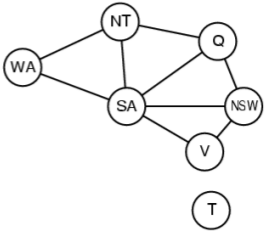
\includegraphics[width=3cm]{constraint.png}
        \caption{Example of constraint graph}
    \end{figure}

 \paragraph{Hypergraph}   An   hypergraph   is   graph   with   ordinary
 nodes (circle)  which   are  the   variable  and  the   constraint,  and
 hypernode (square) which represent the n-ary constraint.

\subsection{Constraint Propagation}

The objective  is to \textbf{reduce the search space}. To achieve  that, we will
try to find  an equivalent CSP to the original one with smaller domains
of variables.

There are two techniques to reduce the size of the domain when considering
constraint \textbf{locally}:
\begin{itemize}
    \item  \textbf{Arc  consistency}  : All the value in variable domain satisfy
        the binary constraint.
      (remove incompatible values in domain)

$X_i$ is arc consistent to $X_j$ if for every value in $D_j$ the is some value in $D_j$ that satisfies binary constraint $(X_i,X_j)$

      $$ X, Y \in \{0,1,\cdots,9\},\quad X=Y^2 \quad \to \quad X \in \{0,1,2,3\} \quad and \quad Y \in \{0,1,4,9\} $$
  \item \textbf{Path consistency} consider constraint between $n$ variables.

        A  two-variable set  ${X_i,X_j}$ is  path consistent  with respect  to a
        third variable $X_m$ if, for every assignment ${X_i=a,X_j=b}$ consistent
        with the  constraint on  ${X_i,X_j}$, there is  an assignment to $X_m$
        that satisfies the constraints on ${X_i,X_m}\quad{X_m,X_j}$

  \item \textbf{Node consistent} All the values in a variable domain
      satisfy the variable unary constraint
\end{itemize}


\paragraph{Bound consistency} It is not always possible to represent the
domain of  each variable as a set. (Ex:  the set \{green,  red, blue\}).
Instead domains are represented with a lower- and upper-bound and are
managed by bound propagation.

For both the lower-bound and upper-bound value of $X$, for every variable Y there
exists some value of Y that satisfies the constraint between X and Y.

\paragraph{Global constraint}  Constraint involving an arbitrary number
of variable and ad-hoc specialized method (ex: Alldiff(X1,X2,..,X8))

\subsubsection{Arc-consistency algorithm}

\begin{itemize}
    \item Start queue with a init arc
    \item While ($X_i, X_j$) in queue :
        \begin{enumerate}
            \item if \textsc{revisite} then
                \begin{enumerate}
                    \item for each $X_k$ in $X_i.NEIGHBORS - \{X_j\}$ add ($X_k, X_i$) in queue
                \end{enumerate}
       \end{enumerate}
\end{itemize}

\textsc{Revisite} delete value in $X_i$ that not satisfy a constraint between $X_i$ and $X_j$

\paragraph{Complexity} \textit{time complexity} of $O(n^2 d^3)$

\subsection{Backtracking Search for CSPs}

\subsubsection{Incremental formulation of CSP search }
\begin{itemize}
	\item The initial state is an empty assignment
	\item The successor function assign a value to an unassigned variable provided no constraint violated
	\item The goal test check if the assignment is consistent and complete
	\item There is a constant value per step. (Path is irrelevant)
\end{itemize}

\paragraph{Commutativity} order the of application  of any given set of
action has no effect on the outcome.

The \textbf{search tree} have a depth of $n$ (number of variables) and the
number of states =  $O(d^n)$ with $d$ the size of the domain.

Because there are $d$ values for $n$ variables we can expect a search tree
with $n! d^n$  \footnote{Branching factor on the top is $nd$, at the next
level $(n-1)d$,\ldots} leaves with only $d^n$ possible assignment.

\subparagraph{\textbf{How}}  with  CSP  search  algorithms  should  only
consider  a single variable for successors  at each node because with
\textbf{commutativity} when assigning values to variables, we reach the
same partial assignment regardless of order.


\subsubsection{Backtracking search}  It's a  \textbf{depth first search}  that choose
values for one variable at a time  and backtracks when a variable has no
legal values left  to assign.

When  choosing variable  in order,  it's  not efficient.  To reduce  the
search,  we  will improve  the  way  we  choose  the variable.  This  is
\textbf{variable ordering}.

\subsubsection{Variable ordering}
It exists two ideas:
\begin{itemize}
    \item \textsc{Minimum Remaining Value}: we choose the variable with the fewest legal values. (first-fail heuristics)
    \item \textsc{Degree Heuristic}: Choose the variable involved in the
        largest number of constraints (it reduces the branching factor in subtree)
\end{itemize}

\paragraph{Choose value  to assign  for selected  variable}
We must decide the order in which to examine its value.

A  solution is  the \textbf{least  constraining value},  the value  that
rules out the fewest choice for the neighboring variables in the
constraint graph. (We try to not have an empty set value for a variable)


\subsubsection{Interleaving search and inference}
When we make choice of a value for a variable, we have a brand-new opportunity to infer new
domain reductions on the neighboring variables.

To \textbf{reduce the search  space} and be more efficient in  the search, a good
idea is to propagate the information to other constraints.

It  is  done  with  \textit{Forward  checking,  consistency  and  global
constraint}.

\paragraph{\textbf{Forward checking} }
When $X$ is assigned a value $v$:
\begin{itemize}
	\item Look at each unassigned variable $T$ connected to $X$ (with binary constraint).
	\item Remove from the domain of $Y$ the value inconsistent with the value chosen for X.
	\item With MRV, failure occurs if a domain becomes empty.
\end{itemize}

\subsubsection{Intelligent Backtracking}  Instead of backing up to the
preceding variable, we back up to a variable and try another value that
might fix the problem.

To achieve that we keep a \textbf{conflict set} for each value that keep
the assignment that are in conflict with this value.
$$ example  \quad : \{Q=red, NSW=green, V=blue \}$$

With \textbf{backjumping} we go to the most recent variable in conflict
set.

\paragraph{Conflict-directed backjumping}

\todo[inline]{Feel free to contribute}

\subsection{Local Search for CSP}

\subsubsection{Complete state formulation of CSP search }
\begin{itemize}
	\item The initial state has a value for every variable
	\item The successor function changes a value of one variable
	\item The goal test checks if the assignment is consistent and complete
	\item There is a constant value per step. (Path is irrelevant)
\end{itemize}


The initial state assigns a value to every variable and the search
changes a value of one variable at a time.

When choosing a new value the most obvious heuristic is to select the
value that result in the minimum number of conflicts. This is called
\textbf{Min-conflict}

\subsection{Structure of the problem}

\subsubsection{Independent subproblem}

We divide the CSP in \textbf{independent subproblem} (\textit{partition of
variables and constraints}) to form $k$ different CSP.

We can solve them separately and the solution is the union of the different
solution. The \textit{time complexity} is reduced to $O(d^{n/k} k)$

To achieve that, we consider  the \textbf{connected component} of
the constraint graph as a subproblem.

\subsubsection{Tree-structure subproblems}

\begin{description}
    \item[Directed arc consistency] under an ordering of variables $X_1, X_2, \cdots, X_n$
        IF every $X_i$ is arc-consistent with each $X_j$ for $j > i$
    \item[Topological sort] : Ordering of variable such that each variable
        appears after its parents in the tree
\end{description}

\paragraph{Solving} Make the tree-structure \textbf{directed arc consistency} with
a topological sort. Choose a value in each domain to have a solution.

\paragraph{Complexity}
Tree-structure  can be  solve in  \textit{time complexity}  of $\color{red} O(nd^2)$
because any tree  with $n$ nodes has  $n-1$  arcs and we can make a
\textbf{directed arc-consistent} in  $O(n)$ step where we need to check
the arc-consistent in $O(d^2)$.


\paragraph{Removing nodes}
\begin{enumerate}
    \item Choose a cycle subset $S$ (size $c$)
    \item For each possible \textbf{assignement} to the variables
        \textbf{S} that satisfies all constraints on $S$
        \begin{enumerate}
            \item \textbf{Remove} in domain any variable that is
                inconsistent with the assignment of $S$
            \item If CSP has solution, return it with $S$ assignment
        \end{enumerate}
\end{enumerate}

\subparagraph{Bad :} Finding the smallest cutset is NP-hard


\paragraph{Grouping nodes}
\begin{itemize}
    \item Each variable appears in at least one subproblems
    \item Two variables connected by a constraint must appear together
        in at least one subproblem
    \item If a variable appears in two subproblems, it must appears in all
        subproblems on the \textbf{path} to connected these subproblems
\end{itemize}

\paragraph{Solution} Solve one subproblem and the result domain of each
variable is the domain use for the next subproblem.

If a variable has an empty set, problem is unsolvable.

\paragraph{Complexity}
Problem is solved \textit{time} $O(nd^{w+1})$ where $w$ is the tree width.

\subparagraph{Bad :} Finding decomposition with minimal tree is NP-hard


\section{Chapter 7 : Logical Agent}
Achieving a goal frequently requires \textbf{more} than searching : \textit{planning,
reasoning and acting}.

\textit{In which we design agents that can form representations of a complex world, use a process of inference to derive new representations about the world and use these new representation to deduce what to do}

\subsection{Knowledge-based agents}

\textbf{knowledge-based agents} can reasoning with knowledge.

\begin{description}
    \item[Knowledge base] : central component of KBA, this is a set of
        \textbf{sentences}
    \item[Background knowledge] : initial knowledge of KB
    \item[Sentence] : assertion about the world
    \item[Axiom] : A sentence without being derived from other sentences
        (\textit{independent})
\end{description}

\paragraph{Operation on KBA} :
\begin{enumerate}
    \item \textsc{Tell} : add a new sentence
    \item \textsc{Ask} : query what is known
    \item \textsc{Make-percept-Sentence} : construct a sentence asserting that the agent perceived
        the given percept at the given time.
    \item \textsc{Make-Action-Query} : construct a sentence that asks what action should be done at the current time
    \item \textsc{Make-Action-Sentence} : constructs a sentence asserting that the chosen action was executed
\end{enumerate}

There operations involve \textbf{inference} (deriving new sentences from old)

\paragraph{Called agent} is perform in three time :
\begin{enumerate}
    \item Tell the knowledge of KB (\textit{action 1.})
    \item What action should perform (\textit{action 2.})
    \item Tell which action was chosen and agent that executed it (\textit{action 3.})
\end{enumerate}

\paragraph{Knowledge level} : Abstract description of what the agent knows and what his goals are.

\paragraph{Knowledge representation} : The language in which the sentence are represented.

Two approach on how the agent is built :
	\begin{itemize}
        \item \textbf{Declarative approach}:  We only tell the agent what
            it needs to know. Sentences told one by one (\textit{by TELL}) until the agent knows how to operate in its environment.
    \item \textbf{Procedural approach} : We encode desired behaviours directly as program code.
	\end{itemize}
\subsection{Example :The Wumpus World}
A board (grid) with a creature that eat agent. Some cases are pits and we try to find a treasure.
\begin{itemize}
    \item Not fully observable (only local perception)
    \item Deterministic (outcome exactly specified)
    \item Not episodic (Sequential at the level of actions)
    \item Static (Wumpus and pits do not move)
    \item Discrete
    \item Single-agent (Wumpus is essentially a natural feature)
\end{itemize}

\paragraph{ } See page 209-210-211 of the book

\paragraph{ } Knowledge gained in different places at different times must
be combined to draw conclusions


\subsection{Logic}
\begin{description}
    \item[Syntax] : Specify all the sentences that are well formed
    \item[Semantic] : Define the \textit{truth} of sentences respect to each
        possible world (interpretation)
    \item[Interpretation] : mathematical abstraction of a possible world
    \item[Model of sentence $\alpha$] is an interpretation where the sentence
        is true.
    \item[M($\alpha$)] : set of all model of $\alpha$
    \item[$KB \models \alpha$] : $\alpha$ is true if KB is true
    \item[$KB \vdash \alpha$] : We can prove $\alpha$ with KB
\end{description}

\subsubsection{Entailment}
$$\textrm{Entailment between } \alpha \textrm{ and } \beta
\quad \equiv \quad \alpha \models \beta  \quad IFF \quad M(\alpha) \subset M(\beta)$$
$\beta$ is true in every model of $\alpha$ (example $x=0 \models xy=0$)

\begin{figure}[!ht]
    \centering
    \begin{tabular}{cc}
        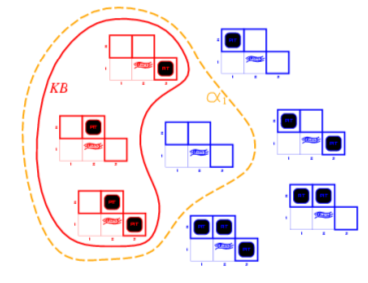
\includegraphics[width=6cm]{alpha_1.png}
        &
        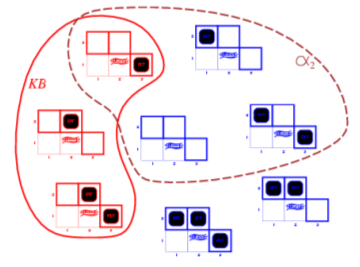
\includegraphics[width=6cm]{alpha_2.png}
        \\
        $\alpha_1$ = ``No pit in 1,2''
        &
        $\alpha_2$ = ``No pit in 2,2''
        \\
    \end{tabular}
    \caption{Wumpus models conclusion}
\end{figure}

If $KB \models \alpha_1$ we can conclude that $\alpha_1$ is true!


\paragraph{To verify $KB \models \alpha$} use \textbf{model checking}.\\
\begin{tabular}{m{11cm}m{1cm}m{1.5cm}m{1cm}}
    \begin{itemize}
        \item enumeration of the interpretations
        \item Find the interpretations which are models of $\alpha$
        \item Check that $\beta$ is these models $\color{red} \alpha \vdash \beta$ ($\beta$ derived by
        $\alpha$)
    \end{itemize}
    &
    \textcolor{red}{Completeness}
    &
    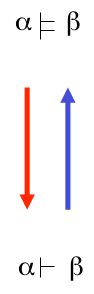
\includegraphics[width=1cm]{soundness.png}
    &
    \textcolor{blue}{Soundness}
    \\
\end{tabular}


\subsection{Propositional Logic}

\subsubsection{Syntax}
$\neg$,
$\wedge$,
$\vee$,
$\Rightarrow$,
$\Leftrightarrow$.

\subsubsection{Semantic}
With \textit{truth table}

\begin{figure}[!ht]
    \centering
    \begin{tabular}{|c|c||c|c|c|c|c|}
        \hline
        P & Q & $\neg P$ & $P \wedge Q$ & $P \vee Q$ & $P \Rightarrow Q$ & $P \Leftrightarrow$ \\
        \hline
        F & F & T & F & F & T & T \\
        F & T & T & F & F & T & F \\
        T & F & F & F & F & F & F \\
        T & T & F & T & T & T & T \\
        \hline
    \end{tabular}
    \caption{Truth table}
\end{figure}


\subsubsection{Simple inference}
Goal is to decide whether $KB \models \alpha$.
\textbf{Model-checking approach} :
\begin{enumerate}
    \item Enumerate the interpretations ($2^n$ where $n$ is the number of symbol)
    \item Check whether $\alpha$ = $P_{1,2}$ is true in every model of KB
\end{enumerate}

The algorithm is \textit{sound} because it implements directly the
definition of entailment and \textit{complete} because it works for any $KB$ and $\alpha$.

\paragraph{Complexity} \textit{time} complexity is O($2^n$) and \textit{space} complexity
O($n$) because it's a \textcolor{red}{depth-first}.


\paragraph{} Note that propositional entailment is co-NP-complete so every
known inference algorithm for propositional logic has a worst-case complexity that is exponential in
the size of the input.

\subsection{Propositional Theorem Proving}

\begin{description}
    \item[Logical equivalence] : $\alpha \equiv \beta$
    \item[Valid] : true in all interpretation
    \item[Satisfiable] : true in some interpretation
    \item[Unsatisfiable/Inconsistency] : always false
    \item $\alpha \models \beta \quad IF \quad (\alpha \wedge \neg \beta)$ is unsatisfiable
\end{description}

\subsubsection{Inference proof}
$$ \frac{\alpha \Rightarrow \beta, \quad \alpha}{\beta} \quad \textrm{ Modus Ponens}, \quad
\frac{\alpha \wedge \beta}{\alpha} \quad \textrm{ And-elimination}, \quad
\frac{\neg (\alpha \wedge \beta}{\neg \alpha \vee \neg \beta} \quad \textrm{ Two sens De morgan}$$

\textit{See all inferences on page 222-223}

\paragraph{Search algorithm} can be used to find a sequence of steps that constitutes a proof.
We just need to define :
\begin{itemize}
    \item \textsc{Initial State} : the initial knowledge base
    \item \textsc{Actions} : The set of actions is all the inferences rules
    \item \textsc{Result} : The result of an action is to add the sentence in the bottom half of the inference
    rule
    \item \textsc{Goal} : Contains sentence we are trying to prove
    \item \textsc{Path cost} : The number of inference rules applied
\end{itemize}

\subparagraph{\textbf{Monotonicity}} is a property of logical systems.
Set of entailed sentences can only \textbf{increase} as information is
added to the knowledge base.
$$ IF \quad KB \models \alpha \quad THEN \quad KB \vee \beta \models \alpha$$

This knowledge might help the agent to draw additional conclusion but it
cannot invalidate any conclusion $\alpha$ already inferred.


\subsubsection{Proof by resolution}
The resolution inference rule need to be sound and complete and use with a
complete search algorithm.
$$ \frac{A \wedge B \vee C, \neg B}{A \vee C}$$

\begin{figure}[!ht]
    \centering
    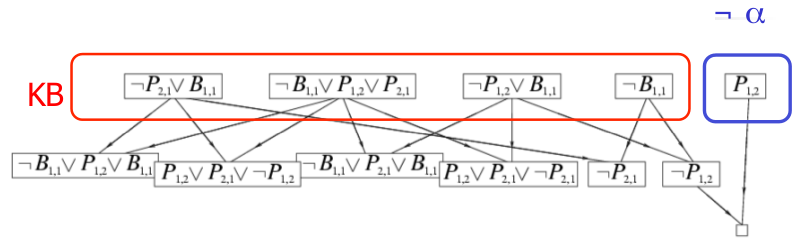
\includegraphics[width=12cm]{proof.png}
    \caption{Proof example}
\end{figure}

\paragraph{Conjunctive normal form}
$$(l_{1,1} \vee \cdots \vee l_{1,k}) \wedge \cdots \wedge (l_{n,1} \vee \cdots \vee l_{n,l})$$

Every sentence of propositional logic is logically equivalent to a
conjunction of clauses using these steps :
\begin{enumerate}
    \item Eliminate $\Leftrightarrow$
    \item Eliminate $\Rightarrow$
    \item Move $\neg$ inside
    \item Distribute $\wedge$ over $\vee$
\end{enumerate}

\paragraph{A resolution algorithm}
This algorithm proves by contradiction $(KB \wedge \neg \alpha)$ because $$KB \models \alpha \quad
 IF \quad (KB \wedge \neg \alpha)$$

For each pair of clauses, we resolve them (use inference rule).  If an
\textbf{empty clause} is derived, then the sentence is unsatisfiable and $KB \models \alpha$
is \textbf{true}

\paragraph{Completeness of resolution}
Resolution is \textbf{complete} because if a set of clauses is unsatisfiable, then
the resolution closure of those clauses contains the empty clause.


\subsubsection{Horn clauses an definite clause}
\begin{description}
    \item[Definite clause] : a disjunction of literals of which exactly one is positive
        ($\neg L_1 \vee \neg Breeze \vee B_{1,1}$)
    \item[Horn clause] : a disjunction of literals of which at most one is positive
    \item[Goal clause ] : a disjunction of no positive literals
\end{description}

Knowledge base containing only \textbf{definite clause} for three reasons :
\begin{enumerate}
    \item Every finite clause $(\neg L_1 \vee \neg Breeze \vee B_{1,1})$ can be write as an
        implication$(L_{1,1} \wedge Breeze) \Rightarrow B_{1,1}$
    \item Inference with Horn clauses can be done through the \textit{forward-chaining} and
        \textit{backward-chaining}
    \item Decide \textbf{entailment} with horn clause can be done in time
        that is \textit{linear} with the size of KB
\end{enumerate}

\subsubsection{Forward and backward chaining}

\begin{figure}[!ht]
    \centering
    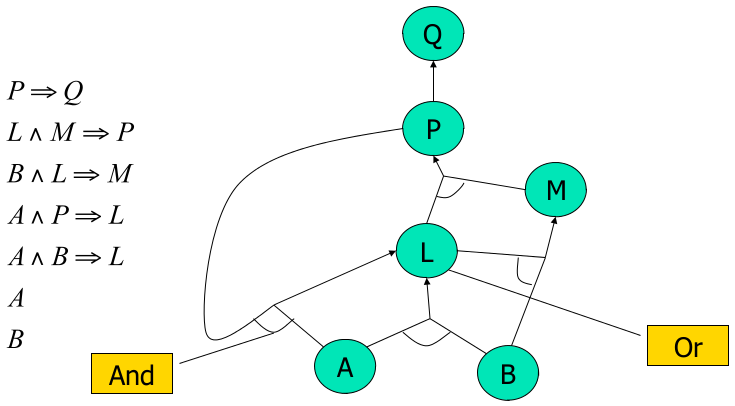
\includegraphics[width=10cm]{andor.png}
    \caption{A set of horn clause with the corresponding \textsc{and-or} graph}
\end{figure}


See the example in the appendices.

\paragraph{Forward}
We start on the known leave (Here A and B). From A and B, we have L. After we cross on the graph
and when a \textit{literal}, q,  is reached then $KB \models q$.

It's easy to see that every definite clause in the original KB is true
for this model.

In conclusion, to prove $KB \models q$, a forward chaining is perform
with the KB and q. If q is reached then $KB \models q$

\paragraph{Backward}
It's the same idea but we start on sequence q (that we suppose this one true) and
we go-back.

\paragraph{Criteria} \textbf{Soundness} because each inference is essentially
an application of \textit{Modus Ponen}. \textbf{Completeness} because every entailed
atomic sentence will be derived ($KB \models \alpha \to KB \vdash \alpha$)


\subsection{Effective Propositional Model Checking}
The algorithms below are algorithm are for checking satisfiability.

\subsubsection{Algorithm: Davis-Putman}
It's like a Model-checking but he use only a \textbf{CNF} input sentence.

Improvement :
\begin{itemize}
    \item \textbf{Early termination} : when a literal is true in the clause then
        the clause is true.
    \item \textbf{Pure symbol heuristic} : a literal is pure if it appears always with
        the same \enquote{sign}. Note that we ignore the sentences already true.
    \item \textbf{Unit clause heuristic} : it's a clause with one literal.
        It must be true and with this assumption other sentence can be simplified
        $$ \frac{B, \quad (\neg B \vee \neg C)}{\neg C} \textrm{ A now C is a unit
        clause where we can be the same}$$
\end{itemize}

\subsubsection{Local search algorithm}
\textbf{WalkSAT} is a local search.
\begin{enumerate}
    \item Start with all variables assigned
    \item Pick a clause false in model :
        \begin{itemize}
            \item Change the value of a randomly chosen variable
            \item \textbf{OR} Change value of the variable that maximizes
                the number of satisfied clause
        \end{itemize}
\end{enumerate}

\paragraph{Return value}
If a model is returned then the input sentence is satisfiable
else if failure is return \textit{failure} then the sentence is
unsatisfiable or we need to give more time

$\to$ use to indicate that sentence is unsatisfiable but it is not a proof!

\subsubsection{Landscape of random SAT problem}

\todo[inline]{see books pg 235}

\subsection{Agent based on propositional logic}
\todo[inline]{example with Wumpus World see slide 7.96}

\section{Chapter 8 $\backslash$ 8.3.3 : First-Order Logic }

\subsection{From Propositional logic to First-Order logic}

 Propositional logic :
 \begin{itemize}
     \item is \textbf{Declarative} : relationships between variables are described through sentences
     \item is \textbf{Excpressive} : can present partial information using disjunction
     \item \textbf{Lacks expressiveness}  power to describe the environment
         concisely (ex: cannot say \enquote{pits cause breezes in
         adjacent squares}).
\end{itemize}

 Then we use \textbf{First-Order logic}, it assumes the world contains:

	\begin{itemize}
		\item Object: people, houses, numbers,\ldots
		\item Relation: unary (red, \ldots), n-ary (bigger than, inside, \ldots)
            $$\textrm{Ex: brotherhood relation is the set } \{<richard, john>, <john, richard>\}$$
		\item Function: successors, father\_of,...
            $$\textrm{Ex: leftleg function } <richard> \to richard leftleg$$
	\end{itemize}

\subsection{Syntax and semantics of FOL}
The \textbf{domain} of a model is the set of objects it contains.\\

	\begin{figure}[!ht]
		\centering
		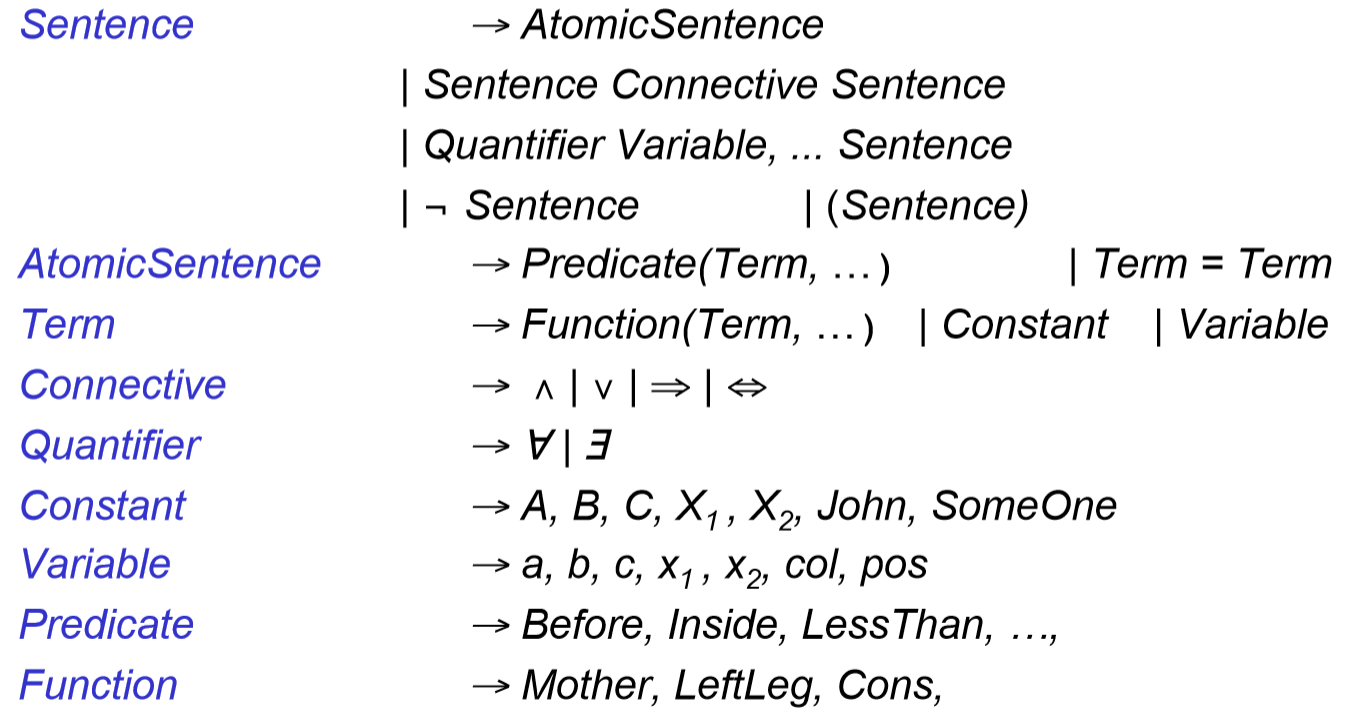
\includegraphics[width=10cm]{fol_bnf.png}
		\caption{Syntax of FOL}
	\end{figure}

 The semantics is provided by interpretation for the basic constructs.

 \begin{tabular}{m{7cm}m{1cm}m{6cm}}
     \begin{itemize}
         \item \textsc{Alphabet} = variables, constants, function symbols, predicate symbols and
             connectors, punctuations and quantifiers
         \item \textsc{Term} = Combination of the alphabet
         \item \textsc{Well-formed formula}
     \end{itemize}
     &&
     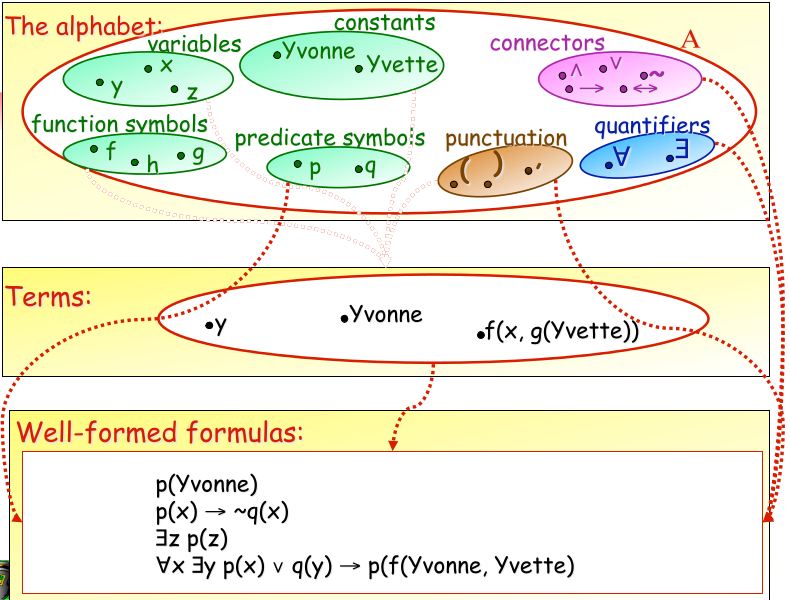
\includegraphics[width=6cm]{fol.png}
 \end{tabular}


 The interpretation maps \textbf{constant, function symbols and predicat symbols}
 to the domain.

 \begin{figure}[!ht]
     \begin{tabular}{m{7.5cm}m{1cm}m{8cm}}
     \begin{itemize}
         \item \textcolor{blue}{D} the domain
         \item \textcolor{red}{function} that maps constants to D
         \item \textcolor{purple}{function} that maps functions symbols to
             \textcolor{orange}{functions: D$\color{orange}\to$ D}
         \item \textcolor{green}{function} that maps predicate symbols to
             \textcolor{brown}{functions: D$\color{orange}\to$ Booleans}
     \end{itemize}
     &&
     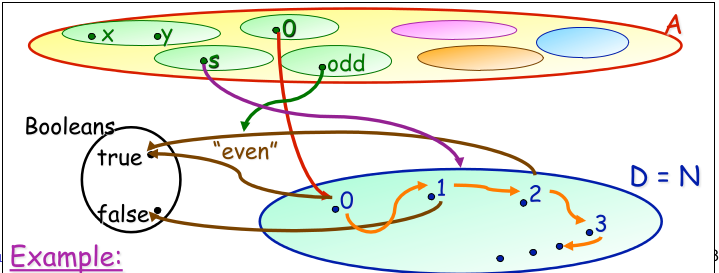
\includegraphics[width=8cm]{fol_inter.png}
 \end{tabular}
 \caption{Interpretation}
 \end{figure}

 \subsubsection{Assigning truth values}

 For closed well-formed formulas F (no non-quantified variable )

	\begin{itemize}
		\item $\forall x$ F(x) is true if $\forall d\in D$,I(F(d)) = true
		\item $\exists x$ F(x) is true if $\exists d\in D$,I(F(d)) = true
	\end{itemize}



    \subsubsection{Quantifiers}

 With  FOL  we  can  use the  quantifier($\forall,\exists$)  to  express
properties of collections of objects.

	\begin{itemize}
		\item $\forall x\quad Human(x) \Rightarrow Mortal(x)$
		\item $\exists x \quad Bird(x) \wedge \neg Can-Fly(x)$
	\end{itemize}

    Take  \textbf{care}  the  order  of  the  quantifiers is  important.  We  can
 express  complex  sentences  with  multiple variables  and  by  nesting
 quantifiers (using several variables instead of several same quantifier).

 The  connection  between  the  two quantifiers  is  defined  as  follow:
 \begin{itemize}  \item $\forall\quad  \neg  P(x)  \equiv \neg\exists  x
 \quad P(x) $  \item $\forall\quad P(x) \equiv \neg\exists  x \quad \neg
 P(x)$ \end{itemize}

\subsection{Using FOL}

 Sentences are added in the KB with \textit{TELL} (ex:
 Tell(KB,King(John))). Queries are made to the KB with \textit{ASK} (ex:
 Ask(KB,King(John))), it will return a list of variable/term pairs that
 satisfies the query.

 \paragraph{Family Relationships}  It's a domain that contains fact of
 familial relation.  A typical sentence for the Wumpus world is like,
 Percept([Stench,Breeze,Glitter,None,None],t).  We use $t$ to represent
 times.

\subsection{Knowledge Engineering}

	Conception and construction of a knowledge base, it's done in several steps:
	\begin{multicols}{2}
		\begin{enumerate}
			\item Identify the task
			\item Assembly the relevant knowledge
			\item Decide on a vocabulary
			\item Encode general knowledge
			\item Encode description of specific problem instance
			\item Use inference procedure to answer queries
			\item Debug the knowledge base
		\end{enumerate}
	\end{multicols}

\subsection{Some complements on FOL}
	\begin{itemize}
		\item The set LC $(\alpha)$ is the set of logical consequences for a sentence $\alpha$.
            $$\beta \in LC(\alpha) \quad IFF \quad \alpha \models \beta. \quad (LC(\alpha) \textrm{ is computable)}.$$

		\item IC $(\alpha)$ is the set of intended consequences for a sentence $\alpha$.
            $$\beta \in IC(\alpha) \quad IFF \beta \quad \textrm{ is true in the intended model. } \quad (IC (\beta) \textrm{ is not computable. })$$
	\end{itemize}

\todo[inline]{See slide 8.49-8.58}

\section{Chapter 9 : Inference in First-Order Logic }

Two approaches to resolve, from FOL to propositional logic or directly
with FOL.

\subsection{Propositional vs FOL inference}

\paragraph{Universal   Instantiation}   For   any   sentence   $\alpha$,
variable $v$, and ground term $g$:   $$\frac{\forall    v\quad
\alpha}{subst({v/g},\alpha)} \textrm{ ,  It means that v  can be replace
with any instance.} $$

  Ex:   from   $\forall    x\quad   King(x)\wedge   Greedy(x)\Rightarrow
  Evil(x)\quad   $   we  can   infer   $\quad   King(  Richard)   \wedge
  Greedy(Richard) \Rightarrow Evil(Richard)$

\paragraph{Existential   instantiation}  For   any  sentence   $\alpha$,
variable $v$ ,and new constant symbol $k$:
$$\frac{\exists\quad\alpha}{subst({v/k},\alpha)} \textrm{, It means that
v can be replace with a new symbol.} $$

  Ex:   from   $\exists   x\quad   mother(Richard,x)$   we   can   infer
  mother(Richard,ANewMother), ANewMother is a Skolem constant.

With these two instantiations, we  can reduce FOL to proposition symbols.
The problem  is that  with function symbols,  there are  infinetly many
ground term (ex:Father(Father(John))).

\subsubsection{Reduction technical issue}

The problem comes from function symbols, there are infinitely many ground
terms.

\paragraph{Theorem Herbrand} If a sentence $\alpha$ is \textbf{entailed} by a FOL
KB, $\alpha$ is entailed by a finite subset of the propositionalized KB.

\paragraph{Application} For n = 0 to $\infty$ do
	\begin{itemize}
        \item create a propositional KB  by instantiating with depth-n terms.
(Father(a),Father(Father(a)),...)
		\item see if $\alpha$ is entailed by this KB.
	\end{itemize}

 If $\alpha$ is not entailed, the algorithm loops.

\paragraph{Theorem Turing} Entailment for FOL is semidecidable

\subsection{Unification}

\paragraph{Unification}   Substitution  that   make  different   logical
expression look identical.
	\begin{itemize}
          \item knows(John,x),knows(y,Bill) by unifying we have the substitution
        $\theta$ = {x/Bill,y/John}
	\end{itemize}

\paragraph{Most General Unifier} The  substitution that makes the least
commitment about the binding variable.
$$ Unify (Parent(John, x), Parent(y,z)) = {y/john, x/z}$$

\paragraph{Standardize apart} If two sentences share variables, we can't
unified them. To avoid name clashes, we rename one of the variable.

\subsection{Forward chaining}
	\begin{itemize}
		\item Find all rules with satisfied premises
		\item Add their conclusions to known facts
		\item Repeat until query is answered or no new facts are added
	\end{itemize}

\paragraph{Generalized Modus Ponens}
$$\frac{p'_1,p'_2,...,p'_n,(p_1\wedge     p_2\wedge    ...\wedge     p_n
\Rightarrow q)}{q\theta} \quad where \quad p'_i\theta=p_i\theta \textrm{
for all i and } \theta \textrm{ is a subsitution.} $$

GMP  used with  KB of  definite clause(only  one positive  literal) and
there is the \textit{assumption} that all variables are universally quantified. It
is \textbf{sound}

\subsubsection{Analysis}

\paragraph{Soundness}  It only derives sentences that are entailed,
because Generalize Modus Ponen does.

\paragraph{Completeness}  It  answers every query whose answers are
entailed  by the  KB,  but may not terminate  because of the
semidecidability of entailment with definite clauses.

\paragraph{Inefficiency}

The FC have three sources of inefficiency:
	\begin{itemize}
		\item Finding all unifiers is really expensive.
		\item Check every rule on every iteration to check if its premises are satisfied.
		\item Many irrelevant are generated.
	\end{itemize}

\paragraph{Incremental Forward Chaining}
To  avoid repetition,  we use incremental forward chaining where  some
rules generate \textbf{new} information which may permit unification of existing
rules. And some rules generate \textbf{preexisting} information that we do not revisit
them when unifying.


\textit{Every new fact inferred on iteration t must be derived from at least one
new fact inferred on iteration t-1}

$\Rightarrow$ At iteration $t$, we check rule only if its premise includes a conjunct
$p_i$ that unifies with a fact $p_i'$ newly inferred at iteration $t-1$.

\paragraph{Algorithm :Rete} It preprocesses the set  of rules in the KB to
construct a sort  of dataflow network in  each node is a  literal from a
rule premise. (see pg 341)

\paragraph{Magic Set}  To avoid generating irrelevant facts, we rewrite
the rule set using  information from  the goal,  so that  only relevant
variable  bindings (belonging  to  a \textbf{magic  set})  are considered  during
forward inference.


\subsection{Backward chaining}

Start with the premises of the goal
	\begin{itemize}
		\item Each premise must be supported by KB
		\item Start with first premise and look for support from KB
	\end{itemize}

    The  \textbf{Backward  chaining}   for  FOL  is  a   function  as  a
depth-first on a And-Or tree.

\subsubsection{Logic programming : Prolog}
TODO

\paragraph{Goal tree} The tree is a bit different as the arc are
OR and the node are a list of goals.

\subsection{Resolution}
Every sentence of FOL can  be converted into an inferentially equivalent
\textbf{CNF} sentence. Different step are used:
	\begin{enumerate}
		\item Eliminate implications
		\item Move $\neg$ inwards
		\item Standardize variables
        \item Skolemization (change existential quantifiers) (\textbf{see below})
		\item Drop universal quantifiers left
		\item De Morgan
	\end{enumerate}

\paragraph{Skolemization} Remove existential quantifiers by replacing
variable with  brand new  constants.

(ex: $\exists  x \quad Q(x)$  becomes Q(A) where  A is unique).

For more complex sentences, we  use function symbol (Skolem Functions) to
indicate the specific value.

(ex: $\forall Animal(x, A)$ become $\forall Animal(x, F(x))$)

\subsubsection{Resolution inference rule}
For $p_i$ and $q_i$ where UNIFY($p_j, \neg q_k$) = $\theta$ :
$$ \frac{p_1 \vee \cdots p_j \cdots \vee p_m, \quad q_1 \vee \cdots q_k \cdots \vee q_n}
{SUBST(\theta, (p_1 \vee \cdots p_{j-1} \vee p_{j+1} \cdots \vee p_m \vee q_1 \cdots q_{k-1}
\vee q_{k+1} \cdots q_n))}$$

\paragraph{ } $\alpha$ is a logical consequence of KB if $KB \models \alpha$
IFF $(KB \wedge \neg \alpha) unsatisfiable$


So we just transform $\neg \alpha$ into CNF and show $KB \wedge \alpha$ unsatisfiable
because after apply resolution rule

\paragraph{}
The resolution is done using inference rule, what follows is an example:\\
$$\frac{P(x,A)\vee Q(x) \vee R(x,y), \neg P(B,z)\vee S(z)}{Q(B) \vee R(B,y)\vee S(A)}\quad with\quad \theta
= {x/b,z/A}$$

To prove that a sentence $\alpha$ is a logical consequence of KB we show
that KB $\wedge\neg\alpha$  is unsatisfiable. We derive until we get an
empty clause (as with propositional logic). Answer for a goal can be
either a Yes/no or a substitution.


\paragraph{Properties of Resolution} It is sound and complete (\textit{see pg 356 for proof})

\paragraph{Introducing answers}
If goal is Kill(curiosity, cat) a \textbf{yes/no} answer is OK.

But if the goal is $\exists x Kill(x, cat)$ we want to have
\enquote{curiosity}, so we stop with the clause Answer($\alpha$) and
$\alpha$ is the answer.

\paragraph{Theorem provers}

\todo[inline]{Feel free to contribute}

\section{Chapter 10 : Classical Planning }

\subsection{Definition of Classical Planning}

Planning is a combination of various IA techniques :
\begin{multicols}{2}
\begin{itemize}
    \item Searching (uninformed and informed)
    \item CSP
    \item Propositional logic (modelling and inference)
    \item FOL (modelling)
\end{itemize}
\end{multicols}

Environment is \textbf{fully observable, deterministic, finite, static, discrete}.

Like a \textit{search problem}, planning define initial state, actions available in a state,
result of action and goal state.

\begin{figure}[!ht]
    \centering
\begin{tabular}{ccc|c}
    Input && Output & Difficulties \\
    \hline
        Set of world state &&& Size of search tree \\
        Action operators &$\to$& Ordering of actions & Search method\\
        Initial world state &&& Difficult to introduce problem decomposition \\
        Goal && \\
\end{tabular}
\caption{Planning}
\end{figure}

\subsubsection{Planning Domain Definition Language}

\textbf{Planning domain  definition language}  allows us to  express all
the actions with one action schema.

\paragraph{\textbf{State}} is a conjunction of (ground and function free) atoms.
\textit{(Note : $\{A, B\}$ i.e. $A \wedge B$ )}
$$ At(Plane1, Melbourne) \wedge In(Plane1, Robert) $$

\textsc{Close world assumption :} no information on $p(a)$ means $p(a)$ false

\paragraph{\textbf{Action}} specified with \textbf{signature} (name and parameter),
\textbf{precondition} (conjunction and disjunction of literals),
\textbf{effect} (conjunction of literal).

\subparagraph{ } An action is \textcolor{red}{applicable} in any state
satisfying its preconditions.

In more details, an action can be executed on a state $S$ if $s$ entails the
preconditions of $a$. $s \models q$ if and only if every positive literal
$q$ is in $s$ and every negative literal $q$ is not in $s$.


\paragraph{\textbf{Result}} is a state which result in the application of a action on a state.

The result is specified by what has changed, everything that didn't change is left unmentioned.


\paragraph{\textbf{Goals}} is a partially specified state like a precondition it's
a conjunction of literals.
A state satisfies a goal is it contains all the atoms of the goal.


\subsubsection{Complexity of classical planning}
\begin{description}
    \item[PlanSAT] : ask whether there exists any plan that solves a planning problem
    \item[Bounded PlanSAT] : ask whether there is a solution of length $k$ or less
\end{description}

\paragraph{ } Both problems are \textbf{decidable} (number of state finite) but if we
introduce function symbols on the language PlanSAT become \textit{semi-decidable}.

\paragraph{ } Both problems are on \textbf{PSPACE} (mode difficult than NP) larger than NP

Less difficult if we disallow negative effects ($\to $NP-hard) and negative
pre-condition ($PlanSat \to P$).

For many problem PlanSAt is in P and Bounded PlanSAT is NP-Complete.

\subsection{Algorithm for planning a State-Space search}

Possible to use \textbf{classical state-space search methods} and with
precondition/effects it's to possible to search in either direction :
\textit{forward and backward}

\begin{figure}[!ht]
    \centering
    \begin{tabular}{cc}
        \multirow{5}{*}{
            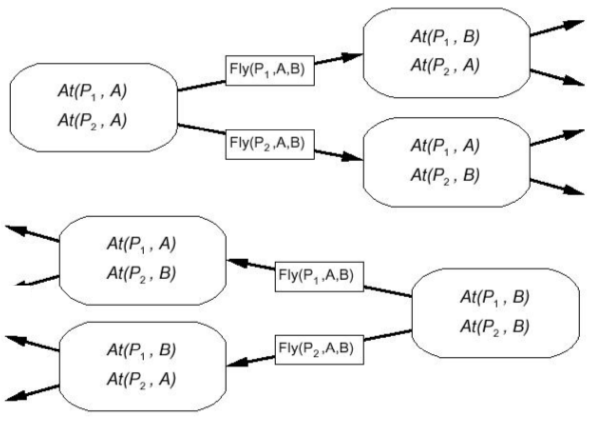
\includegraphics[width=8cm]{state_space.png} }
            & \\& \\& Forward \\ & \\& \\ & \\&\\&
            \\&  Backward \\& \\ &\\
        \end{tabular}
    \caption{Forward and backward state space}
\end{figure}

\subsubsection{Forward state-space search}

Forward  planning  is prone  to  explore  many \textbf{useless}  actions
especially if uninformed. The second problem  is that the state space is
usually  very  large  (\textit{branching factor})  and  a  accurate
heuristic is essential to solving the problem.

\subsubsection{Backward state-space search}

We start  from the goal and  apply the actions backward  until finding a
sequence of steps that reaches the initial state. In general backward
search works only when we know how to regress from a state to
its predecessor which is not always easy.

However with the \textbf{PDDL} representation it is \textbf{easy to make regress actions}.

Backward search keeps the branching factor lower than forward for most
problems but it is harder to find good heuristics.


\subsubsection{Heuristics for planning}

An admissible heuristic can be derived by defining a \textbf{relaxed problem} that
is easier to solve. There are two ways we can relax:
\begin{itemize}
    \item Admissible :

    \begin{enumerate}
        \item \textbf{Adding more edges} to the graph
            making easier to find path or by grouping node together.
            \begin{itemize}
                \item Ignore \textbf{preconditions heuristic}
                \item delete \textbf{negative effect on result}
            \end{itemize}

        \item \textbf{Reduce number state} by mapping many states to one,
           this is done by ignoring some fluents.

       \item \textbf{Monotonic progression} to the goal state done by ignore delete
           lists.
           Assume that all goal and preconditions contain only positive literal.
           (\textit{Approximation is P with Hill-climbing})
    \end{enumerate}

    \item Not admissible, not optimal solution with A* :

        \begin{enumerate}
            \item \textbf{Subgoal independance} :
                A key idea to define  heuristics is decomposition, dividing the problem
                into multiple subproblems and solving each part independently.

            \item \textbf{Set cover} : count the action needed to have the goal test.
                We don't take the optimal solution (because it's NP-hard) but
                we take a solution found

        \end{enumerate}
\end{itemize}


\subsection{Planning graph}
A Planning graph is a sequence of levels of states.

\begin{figure}[!ht]
    \centering
    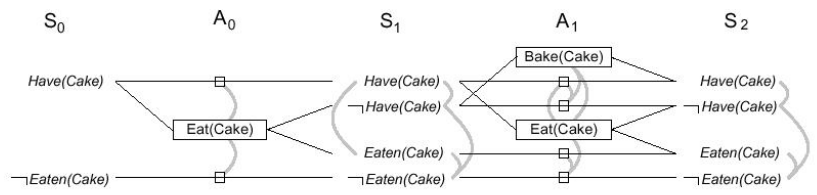
\includegraphics[width=16cm]{planning.png}
    \caption{Planning graph}
\end{figure}

Planning graph can be used to give better heuristics. A planning graph is a
directed graph organized into \textbf{levels}. The first level $S_0$
consists of nodes representing each fluent that holds in $S_0$ then $A_0$
consists of nodes for each possible action applicable on state $S_0$.


$S_i$ contains all the literals that could hold on time $i$ depending on an
action executed at time $i-1$. It is possible to $p$ and $\lnot p$ to both
be present in $S_i$. $A_i$ contains all actions that have their
precondition satisfied at time $i$.

\paragraph{Mutex}

We can add mutex link on a planning graph to represent impossibility of
certain choices between each other. Mutex reduces conflict to \textbf{pair}
of actions (or literals).

There are different kinds of mutex link.

\begin{enumerate}
    \item Between two actions
        \begin{itemize}
            \item \textbf{Inconsistent effects} : one action negates an
                effect of the other action. (Eat(cake) and Have(cake) have
                inconsistent effect because they disagree on have(cake))

        \item \textbf{Interference} : one of the effect of an action is the
            negation of precondition of the other action.

        \item \textbf{Competiting need} : one of the precondition of one
            action is mutually exclusive with the precondition of the other
            action.

        \item \textbf{Opposite literal} : one is the negation of the other on the same level.
        \end{itemize}
\end{enumerate}

Computation of mutex can be efficiently.

\paragraph{Level off}
Is a point in the planning graph where two consecutive levels are identical.

\paragraph{Complexity}
Construct planning  graph is in  polynomial time $O(n(a+l)^2)$  with $n$
level, $l$ literals and $a$ actions.

\subsubsection{Heuristic estimation}
\begin{description}
    \item[Unsolvable] : if any goal literal fails to appear in the final level of graph.
    \item[Level-cost] of literal $g$ : level at which $g$ first appear.
        (\textit{Admissible})
    \item
    \item[Max-level] heuristic : Maximum level cost of the goals. (\textit{Admissible})
    \item[Level sum] heuristic : Sum of the level costs of the goals. (\textit{No admissible})
    \item[Set-level] heuristic : Level at which all the literals in the goal appear
        without any mutually exclusive pair. (\textit{Admissible})
\end{description}

\subsubsection{Algorithm: Graphplan}
Graph is constructed level by level. We also keep hashmap called
\textit{nogoods} (level,set of goals) containing all the goals not achievable in a level.
\begin{itemize}
    \item if graph and nogoods have both leveled off then no solution
    \item if all the goal literals are non mutex in
     current level, then a solution might exist within the current graph
     (Check with extract-solution)
    \item else no solution in current and we expand this one
\end{itemize}

\paragraph{Extract-solution}
Reduce the problem to a backward search problem with boolean CSP
where the variables are the actions at each level. (\textit{true if in the
plan, false otherwise})

\begin{enumerate}
    \item initial state : Last level of the planning graph + set of \textbf{goals}
    \item Operation : choose a (\textbf{conflict free}) subset of actions at the level of
        the state whose effects covers the goals in the state
    \item Goal state : reach a state at level 0 such that all goals are
        satisfied.
\end{enumerate}

\subparagraph{Heuristic guidance}
\begin{itemize}
    \item Pick first literals with highest level cost
    \item Prefer actions with easier precondition
\end{itemize}

\paragraph{Complexity} \textit{time} is polynomial

\subsubsection{Termination of Graphplan}
The graphplan algorithm will terminate when the graph and the nogoods both have level off.
But is it sure that the graph and the nogoods will always level off ?

To prove this, these are certain properties of planning graphs which are monotonically increasing or decreasing.
\begin{itemize}
    \item Literals increase monotonically : Once a literal appears at a given level, it will appear at all subsequent levels.
    \item Actions increase monotonically : Once an action appears at a given level, it will appear at all subsequent levels.
    \item Mutexes decrease monotonically : If two actions are mutex at a
        level $S_i$ they were mutex at all the previous levels where they
        both appear (same for the literal). But if you consider that the
        invisible literals and actions (the one that cannot gold at a level
        $S_i$) are mutex with everything, when you add a action, you reduce
        mutex.
    \item No-goods decrease monotonically : If a set of goals is not achievable at a given level then they are not in any previous level either. But they are achievable at some level
\end{itemize}
Because the actions and literals increase monotonically and because there are only a finite number,
there must come a level that has the same number of actions and literals as the previous one. Because mutex and no-goods decrease, there must come a level that as the same number of mutexes and no-goods (minimum 0). When the graph has reach this state the algorithm is done and we can return failure.

\subsection{Other Classical Planning Approaches}

Here are some other approaches :

\begin{itemize}
\item Translating to a Boolean SAT problem
\item Forward state-space search with carefully crafted heuristics
\item Search using a planning graph
\end{itemize}

\subsubsection{Planning through SAT}
Planning by testing the satisfiability of a propositional sentence. How do
we translate a PDDL description into something that can be used by a SATPlan

\begin{itemize}
\item Initial state: add $F$ for every fluent in the problem initial state and $\lnot F$ for every fluent
not mentioned in the initial state. (PDDL)
\item Propositionalize the Actions.
\item Propositionalize the Goal: for every variable in the goal, replace the literals that contains variables with a disjunction over the constants.
\begin{align}
On(A,x) \land Block(x) \text{ with objects A and B would be} \\
(On(A,A \land Block(A)) \lor (On(A,B) \land Block(B))
\end{align}
\item add successor-state axioms
\item add precondition axioms
\item add action exclusion axioms
\end{itemize}

\subsubsection{Planning with FOL}
FOL has some limitations about the representation of time. It uses a representation called situation calculus to get around the notion of linear time and replace it with the notion of branching situations.

\todo[inline]{This part needs to be completed. Feel free to contribute}


\subsubsection{Planning as CSP}
CSP has a lot in common with SAT, the encoding is similar to the encoding to a SAT problem.
With one simplification, at each time step we only need a single variable, $Action_t$, whose domain is the set of possible actions. We no longer need one variable for every action.


\section{Chapter 11 $\backslash$ 11.2, 11.4 : Planning in the Real World}

Need to addition the duration of tasks  to find a plan  that minimizes the
total time to complete the job.

\subsection{Time, schedule and resources}

\subsubsection{Representing temporal and resource constraints}

\paragraph{Job-shop scheduling}

Set  of  jobs (\textit{jobs  is  a  collection  of action  following  an
order}).

Each action has a duration  time and a set of resources needed.
Resources can be either reusable, consumable or produce via an action.

$\to$ The objective is to find a plan that complete the job.

\paragraph{Makespan} The total duration of the plan.

\subsubsection{Solving scheduling problem}

\paragraph{Critical path} Path whose  duration is the longest. (Delaying
action in the CS  slow down the plan) To minimize  the makespan, we must
find  the earliest  start  times  for all  the  actions consistent  with
ordering constraint.

\paragraph{Slack} $= ES - LS$ where $ES$ is the earliest  possible start time
and $LS$ the latest possible start time.

\subparagraph{ } We  use the \textbf{Critical Path  Method} to determine
the possible start and  end time of each action. This  method is done as
follow ($A\prec B$ means that $A$ comes before $B$):
	\begin{itemize}
		\item $ES(Start) = 0$
		\item $ES(B)=Max_{A\prec B}ES(A)+Duration(A)$
		\item $LS(Finish)=ES(Finish)$
		\item $LS(A)=Min_{B\succ A}-Duration(A)$
	\end{itemize}

We set an ES  value when all the predecessors action have  an ES and we
set that it's the max of the predecessors (Same idea for LS).

\paragraph{Complexity}  The complexity  of  the algorithm  is in  $O(N*b)$
where $N$ is the  number of actions and $b$ is the maximum branching factor
into or out of an action.

To  model the usage of resource,  we add of
the RESOURCE(R1(k),...,Rp(k')) and USE R1(1) description to PDDL. The $k$
is number of instance of the resource.

\subsection{Planning and Acting in Nondeterministic domain}
Some  problem can't  be  resolved with  classical  planning because  the
initial state  can't be fully specified.  That's what happen when the
environment is not deterministic and not fully observable.

\subsubsection{Sensorless planning}
There is  no sensor operator, it uses open world assumption which states
that if a fluent does not appear, its value is unknown.

\todo[inline]{(see pg 424) feel free to add a summary here}

\subsubsection{Conditional planning}
Plan with different branches for  the different contingencies that could
arise. There are sensor operator, and it has a if-elif structure.(see pg
428)

\subsubsection{Replanning}
Same  as  conditional  planning  except that  alternative  plan  can  be
computed at execution time. (see pg 431)

\section{Chapter 18.1-3, 18.10 : Learning from Examples }
\textbf{Learning} improve performances on future tasks after making observations. Learning is nice for multiple reasons : we cannot anticipate
all possible situations, the future tasks may change or the programmer may not be able be to program a function to resolve the tasks by himself.

\textit{We concentrate on learning problems from a collection of input/output,
learn a function that predicts the output for new inputs}

\subsection{Form of Learning}

Three types of \textbf{feedback} that determine the three main types of learning :
\begin{enumerate}
    \item \textbf{Supervised Learning} : agent observes some input-output pairs and learns
        a function that maps from input to output
    \item \textbf{Reinforcement Learning} : agent learns from a serie of reinforcements
        (rewards or punishments)
    \item \textbf{Unsupervised Learning} : agent learns patterns in the input
        even no explicit feedback (output) is supplied.
\end{enumerate}

\subsection{Supervised Learning}

Given a training set $(x_1, y_1),\cdots, (x_n, y_n)$ where $y_i$ is generated by $f(x_i)$
Discover a function \textcolor{red}{h} that approximates f.

(\textit{f can be stochastic and we have to learn his conditional probability distribution.})

\begin{description}
    \item[Hypothesis space] : Set of function where $h$ is taken from. A classical
        hypothesis space is polynomial.

        \textit{Trade-off between the expresiveness of a hypothesis space and the
        complexity of finding a good hypothesis within that space}
    \item[Realizable] : hypothesis space contains the true function.
    In some cases, we can guide the search by telling how probable a
    hypothesis is to be good given the data set. For example degree-1 or degree-2 polynomial function might have a big probability but degree-7 a lower one. This helps reducing the hypothesis space.
 \end{description}

\paragraph{Accuracy} To measure the accuracy of the function \textbf{h} we try it on a test set, which is different from the training set.
A hypothesis \textbf{generalize} well if it correctly predicts the value of $y$ for new examples

\begin{description}
    \item[Classification] : if the output $y$ is taken from a finite set of values
    \item[Regression] : if the output $y$ is a number
\end{description}

\paragraph{Approximate} We always choose the simplest hypothesis consistent with the data
like says \textit{ockam's razo}. $\to$ (a) is thus better than (b).

$$ h* = arg \quad max_{h \in H} \quad P(data|h) . P(h)  \quad \textrm{ where h* is the most probable}\footnotemark$$

\footnotetext{$P(data|h) . P(h)$ is derived by \textit{Bayes rule} from $P(h|data)$ }
In  hypothesis  space, we  give  a high  prior  probability \textbf{P(h)}  for  simple
solution (\textit{degree-1 or -2 polynomial})  and low for hard solution
(\textit{degree-7 polynomial})

\begin{figure}[!ht]
    \centering
    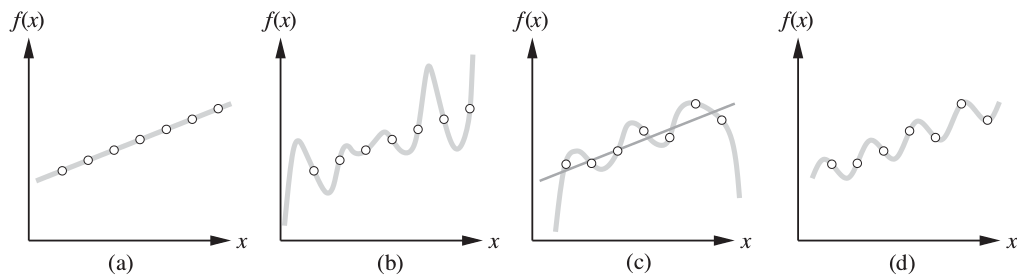
\includegraphics[width=14cm]{razor.png}
    \caption{Approximate a function}
\end{figure}

\subsection{Learning Decision Trees}
A decision tree represents a function that takes as input a vector of
values and returns a decision, a single value. It reaches his decision
by performing a sequence of tests, each node is a test of the value of one of the input attributes and the leaf node specifies the value to be
returned.

In figure ~\ref{decisionTree} you can see a example with the following input:
\begin{enumerate}
\item Alternate: whether there is a suitable alternative restaurant nearby.
\item Bar : whether the restaurant has a comfortable bar area to wait in.
\item Fri/Sat : true on Fridays and Saturdays.
\item Hungry: whether we are hungry.
\item Patrons: how many people are in the restaurant (values are None, Some, and Full ).
\item Price: the restaurant’s price range.
\item Raining : whether it is raining outside.
\item Reservation: whether we made a reservation.
\item Type: the kind of restaurant (French, Italian, Thai, or burger).
\item WaitEstimate: the wait estimated by the host (0–10 minutes, 10–30, 30–60, or >60).
\end{enumerate}

\begin{figure}[!ht]
    \centering
    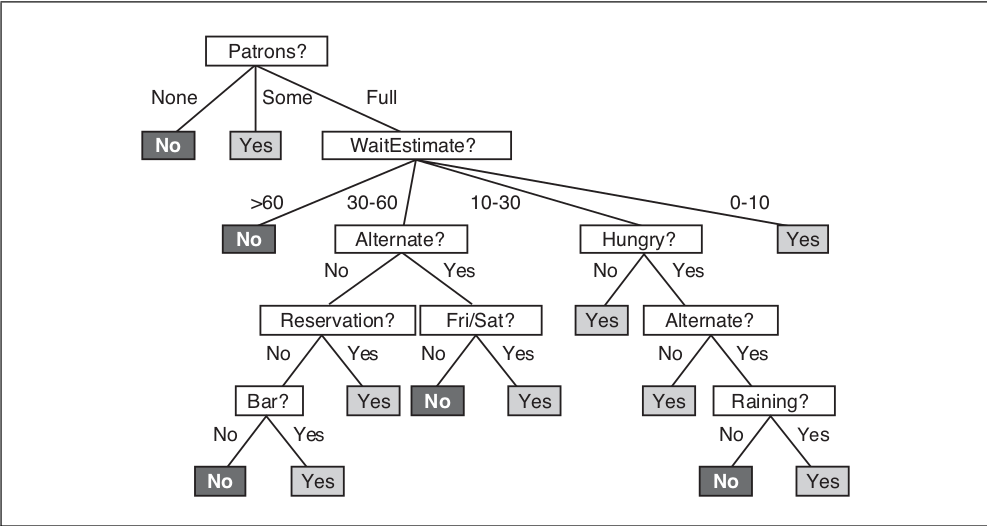
\includegraphics[width=14cm]{decisionTree.png}
    \caption{Decision Tree}
    \label{decisionTree}
\end{figure}

A goal attribute is true if the inputs satisfy one of the paths leading to a leaf which value is true :

\begin{align}
Goal \leftrightarrow (Path_1 \lor Path_2 \lor ... \lor Path_n) \\
Path = ( Patron = full \land WaitEstimate = 0-10 )
\end{align}

\paragraph{How to get the smallest tree possible ?}
With some simple heuristics we can find a approximate solution. The greedy
divide-and-conquer strategy, always tests the most important
attribute first.

\subsection{Decision tree from example}
We can build decision tree from examples, tuples $(x_i,y)$ where $x_i$ are
attributes and $y$ the boolean value. See figure ~\ref{decisionTreeFromEx}
We get a decision tree consistent with the example and as small as possible.

\begin{figure}[!ht]
    \centering
    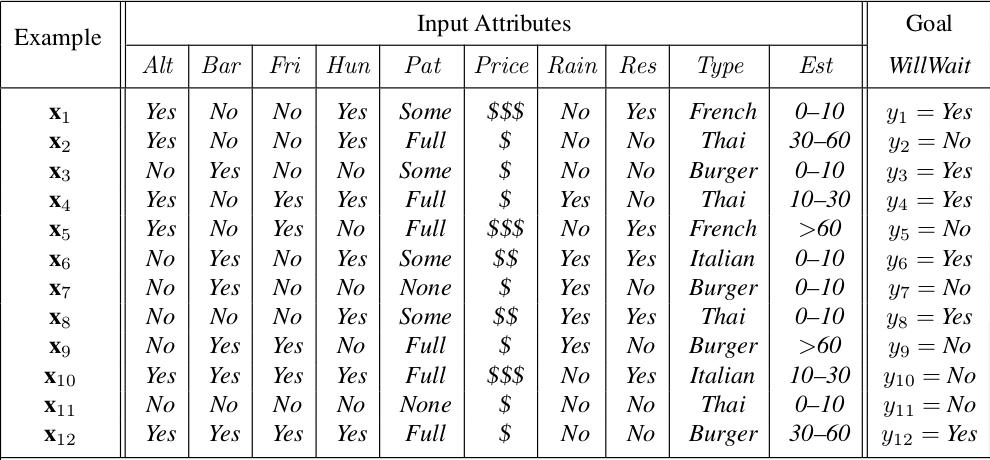
\includegraphics[width=14cm]{decisionTreeEx.png}
    \caption{Decision Tree examples}
    \label{decisionTreeFromEx}
\end{figure}

When build decision tree there is four cases that occurs :
\begin{enumerate}
\item all the remaining examples are positive (or negative). Then we are done.
\item if some are positive and some are negative then we choose the best attribute to split them.
\item if there is no example left, meaning no example have been observed from this situation, return a default value.
\item if there are no attributes left and we still have positive and negative then the examples are inconsistent, return plurality classification.
\end{enumerate}

\subsection{Learning curve}
We split the examples into training set and test set, we learn hypotheses
and measure the accuracy using the test set.
We start with a training set of $1$ and go up to a training set of $n-1$.
We can see that accuracy increases with large training sets.

\subsection{Choosing attribute}
\begin{itemize}
\item Pick the on which will minimize the depth of tree
\item Perfect one, divide example into positive and negative
\item Useless one, device sets with the same proportion of positive and negative
\end{itemize}

\section{Annexe}
%\includepdf{forward_example.pdf}

\begin{thebibliography}{1}
\bibitem{wikiadmheur} http://en.wikipedia.org/wiki/Admissible\_heuristic, {\em Wikipedia}
%\bibitem{Propagation} P.G. Fontolliet, {\em Traité d'Electricité}, Volume XVIII, Ecole polytechnique fédéral de Lausanne, pp 72-73
\end{thebibliography}

\end{document}
